%% move stuff to defs file
\newcommand{\todo}[1]{{\bfseries [[#1]]}}
%% To disable, just uncomment this line
%% \renewcommand{\todo}[1]{\relax}

\documentclass{acm_proc_article-sp}
\usepackage{url}
\begin{document}

\title{A latency-tolerant runtime for large graph computations}

\numberofauthors{7}
\author{
(authors)
}

\maketitle
\begin{abstract}

  Large irregular applications such as sparse, low diameter graph problems often
  perform badly on commodity clusters. These application make many
  non-sequential accesses to global data structures with low degrees of
  locality, interacting badly with commodity processors' memory
  systems, which are optimized for local, sequential memory
  accesses. Special-purpose hardware optimized for these irregular
  applications has been built; the Cray XMT is one such machine. It
  uses multithreading to tolerate the latency of low-locality memory
  accesses, and while it exhibits excellent performance and energy
  efficiency for irregular applications, it performs badly on standard
  sequential applications \todo{Brandon: should this be more specific or worded differently? Its true sequential perform badly since switching between many threads, but also does XMT also perform  poorly (relative to alternatives) on highly parallel but regular apps with lots of temporal and spatial locality?}. We believe we can have the best of both
  worlds: we argue that modern commodity processors have many of the
  features necessary \todo{Brandon: we will have to be able to list these as features in the paper or use a different phrase; my feeling is that these are aspects of the system which are not optimized for this but are sufficient to suggest potential for enough memory concurrency} to give good performance on irregular problems,
  and that a latency-tolerant runtime designed to exploit these
  features can enable speedup for irregular applications on commodity
  processors. In this paper, we describe the key features of such a
  runtime system, and what a cluster built using our runtime might
  look like. Using a preliminary single-node implementation of our
  runtime, we obtained speedups on simple list chasing benchmarks. Our results show promise for a multi-node implementation.

\end{abstract}

\section{Introduction}


Graphs have proven to be a useful abstraction for solving real-world
problems in social and biological network analysis. But many graphs in
social and biological network analysis are sparse, with low diameter
and a degree distribution that follows a power law. These properties
make it difficult to take advantage of the locality assumptions built
into the memory hierarchy of modern processors, so that even simple
traversals are dominated by memory latency.

And these graphs can be large---too large for a single node \todo{may want to avoid saying 'node' since graph 'node' is also used in this paragraph}. In January 2011, Facebook had 500 million active users with an average of
130 friends each \cite{Facebook:2011p91}. A natural approach would be
to try to partition the graph across the nodes in a cluster. But with
low diameter graphs, a traversal starting at any node is likely to
quickly leave its partition and travel over the network, incurring
high latency costs. And power law graphs have a small number of nodes
that generate significantly more work than other nodes, leading to
computational imbalance.

% Facebook's friend suggestion
% algorithm in 2010 ran on a 40-node cluster with 72GB memory per
% node. Even with that capacity, new suggestions could only be computed
% every two days \cite{Backstrom:2010p90}.


Multithreading is a technique that has been used successfully to
implement efficient computations for these graphs. The Cray XMT is an
example of such a solution: it tries to solve the memory latency
problem through concurrency rather than caching. Each XMT processor
supports 128 hardware contexts and $\sim$1000 outstanding memory
operations and is able to switch contexts every cycle. But this
approach has a limitation: each context is significantly slower than a
modern commodity processor, yielding bad single-threaded
performance. While the XMT is fast at sparse, low-degree graph
problems, it is slow at other scientific codes that can take advantage
of commodity processors' memory hierarchies. Thus, few XMTs have been
built.

We want the best of both worlds---we want to build a system that has
good performance on both these low-locality graph codes as well as on
common scientific codes. Our approach is inspired by the XMT, but
implemented in software on commodity microprocessors. The core of our
approach is a lightweight coroutine library designed to overlap
long-latency memory prefetches with other contexts' computation. This
document describes our approach.

\todo{do we want to mention hardware at this point? If so, we should
  perhaps call it a hybrid approach.}

\section{Programming model}

While the ideal programming model is one that facilitates easy
expression in the problem domain as well as efficient execution on the
available hardware, our programming model today is motivated by only
efficient execution: it exists as a rudimentary library for concept
demonstration, not as a language suitable for development.  The
programming model we use today is therefore only partially formed. It
exists as an augmentation of existing threaded programming models such
as pthreads or openmp that are readily available on most computer
systems.

Though not strictly necessary, for ease of exposition we imagine a
one-to-one binding between threads and cores.  Our model manifests
within any thread independently of the others as a ``fray'' \todo{for lack
of better term }.  Within the thread, a fray instance is the
instantiation of a set of coroutines and a scheduler.  Instantiation
is at user-level and the operating system sees the entire fray as as a
single user-level thread.

\todo{ describe calls that perform thread \& scheduler instantiation; and schedule activation }

Each coroutine executes non-preemptively, utilizing the core to which
its ``parent'' thread has been assigned by the operating system until it
reaches a yield point.  Typically, the coroutine yields after
initiating a prefetch operation on data that the programmer or
compiler anticipates would probably not complete before the data is
referenced by a subsequent load operation.  In this way, the core
continues to execute instructions for other coroutines when otherwise
it would likely stall.  The programming model thus tolerates latency.

\todo{ describe calls to prefetch-and-yield }

When a thread frays, for the sake of expediency, a fixed portion of
its stack is divided amongst the coroutines.  Given a finite stack,
each coroutine is constrained to execute a call tree of depth known to
be finite at compilation time: recursion is not yet permitted.

\todo{ discussion of coroutines \& synchronization } Were a coroutine to
block on a synchronization variable shared with other threads, the
entire fray would suspend execution.  This can lead to deadlock when,
for example, one coroutine waits to consume from another thread that
is waiting to consume what only another coroutine in this first fray
can produce.  Instead, coroutines must yield on failed synchronization
events, spinning rather than blocking, where were they bonafide
thereads, blocking might be more efficient.

\todo{ say something about ``synchronization'' within a fray }

Coroutines completing their work yield without adding themselves to
the scheduling queue.  The last coroutine to exit in this way returns
as the main thread, as in the common  fork-join model of parallelism.

many many threads

prefetch and switch on 

full/empty bits 

\subsection{Opportunities}

characteristics:



little FP use ==> don't worry about FP registers

would like enough concurrency to keep pipeline filled, but commodity CPUs don't have enough external bandwidth. So, get enough to saturate bandwidth.



\section{Approach}

Describe general approach, explaining 

\subsection{Low-latency context switch}

switch only stack pointer and program counter; depend on compiler to save/restore anything else. in general case, hopefully this will be fast.

\subsection{Memory concurrency}

Commodity procs don't provide enough. use software? FPGA?

\subsection{Synchronization}

use existing atomic instructions? Use FPGA listening snoops on QPI?


parition remote memory on each node; have one thread access each
partition, making sync easier

\subsection{Extending to a multi-node system}


\section{Current Implementation and Results}

\todo{Begin eval insert}
\section{Evaluation}
\label{sec:evaluation}

The goal of our evaluation is to show that the core pieces of the \Grappa
runtime system, namely our tasking system and the global memory/communication
layer work as expected and together are able to efficiently run irregular
applications. We evaluate \Grappa in three basic steps:

\begin{itemize}

\item We present results that show that the \Grappa runtime is able to sustain
very high concurrency rates and the communication layer is able to sustain a
very high rate of global memory operations. We also show the performance of a
graph kernel that stresses communication and concurrency together.

\item We show how some popular irregular applications running on \Grappa
compare to the Cray XMT and hand-tuned MPI code.

\item We finish with a characterization of system behavior, including
profiling where execution time goes, how aggregation affects message size and
rates, how global memory and work stealing behaves.

\end{itemize}

\subsection{Basic \Grappa Mechanisms}
\label{eval:basic}

\paragraph{User-level context switching.}

As discussed earlier, fast context switching is at the heart of \Grappa's
latency tolerance abilities. We assess context switch overheads using a simple
microbenchmark that has a configurable number of workers, where each worker 
just increments values in a large array. 

\begin{figure}[ht]
    \begin{center}
      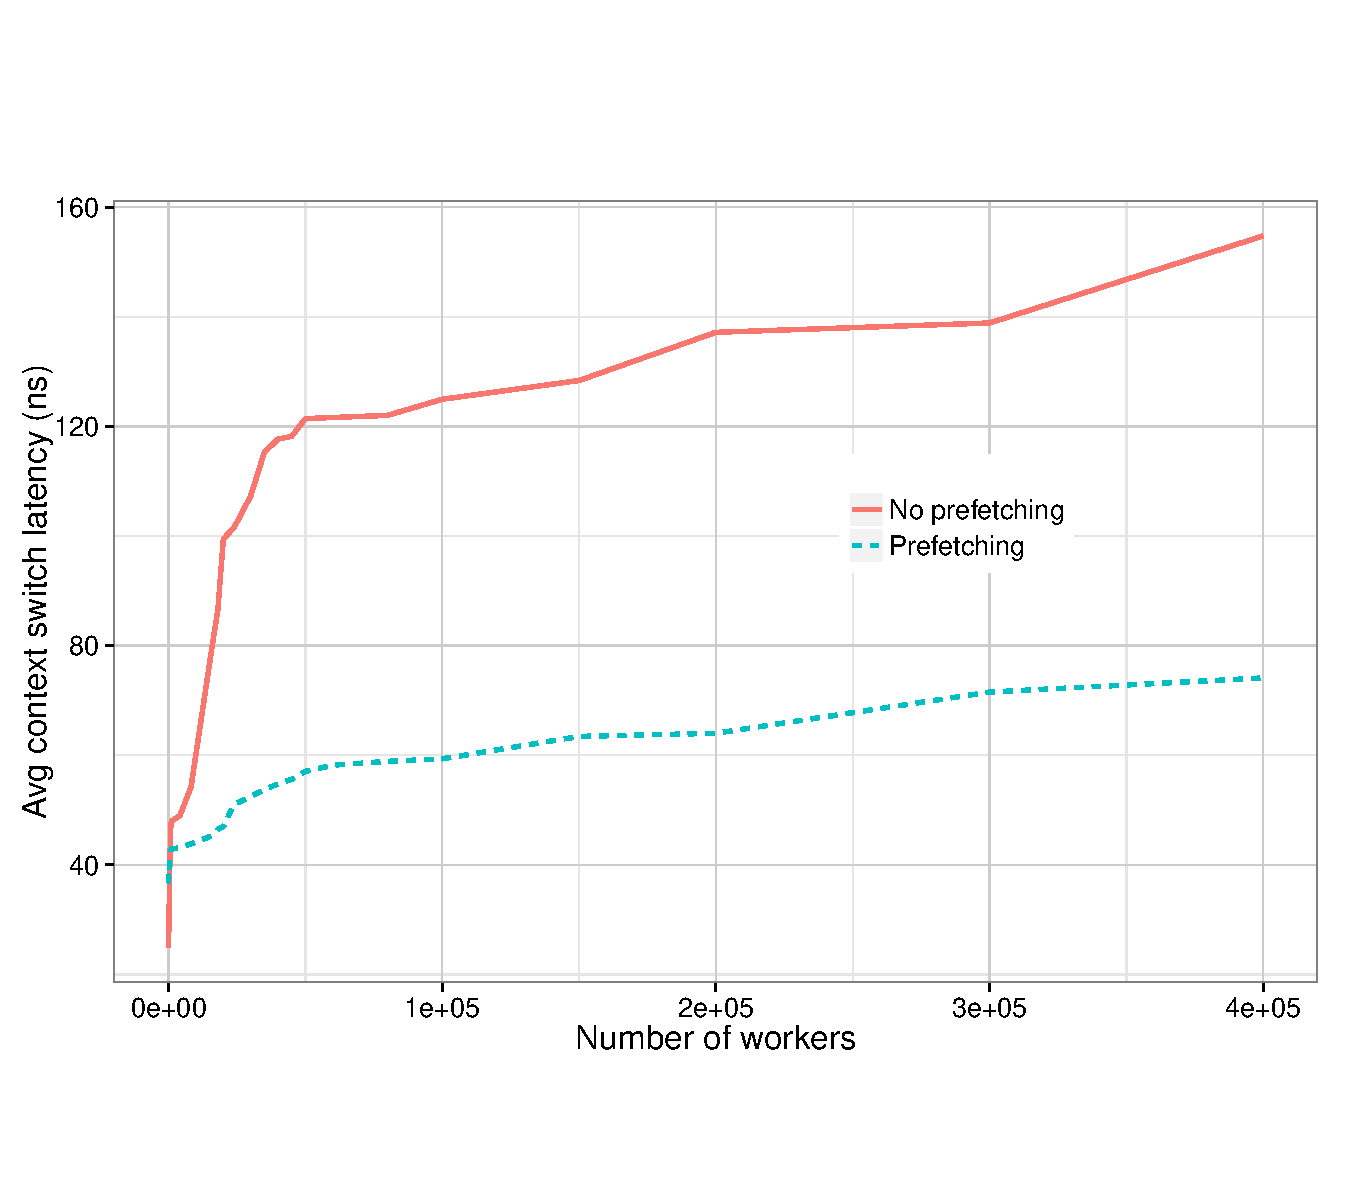
\includegraphics[width=0.5\textwidth]{figs/context_switch_time.pdf}
    \end{center}
    \caption{Average context switch time with and without prefetching.}
    \label{fig:context-switch-exp}
\end{figure}

Figure~\ref{fig:context-switch-exp} shows the average context switch time as
the number of workers grow. There are two important takeaway points from these
data. Context switch time for the number of workers we use ($~$1K workers) is
on the order of 50 ns; and prefetching has significant impact on context
switch time. And context switch time does not grow significantly with the
number of workers --- even with one-half million workers, context switch
is around 75ns.

We also measured (not in the plot) the \emph{rate} of context switch for all
cores in a node, which showed that our rate is limited by off-chip memory
bandwidth. Each context is 4 cache lines (1 for the worker struct and 3 for
stack data), leading to 8 cache line transfers per context switch
(write the previous context, read the next in). The off-chip bandwidth of a
single socket in our system is 270M cache lines per second, which implies that
we can sustain at most 34M context switches per second per socket, which is
almost exactly what we sustain.

In summary, our context switch engine is able to efficiently sustain very high
concurrency and as we will show later, the amount of concurrency sustained is
sufficient the latencies \Grappa needs to hide.

\paragraph{Global memory and communication.} We measure the performance of
\Grappa's global memory and communication layers using a faithful
implementation of the giga updates per second (GUPS) benchmark.
Read-modify-write updates are dispatched at random to a large array. This
benchmark stresses the communication layer of \Grappa separately from the
scheduler, because only a single worker is used per system node.
Figure~\ref{fig:grappa-gups} shows that \Grappa is able to sustain well over a
billion updates per second with 64 nodes. This compares very favorably to
published results~\cite{gups} for other high-end HPC systems.


\begin{figure}[ht]
    \begin{center}
      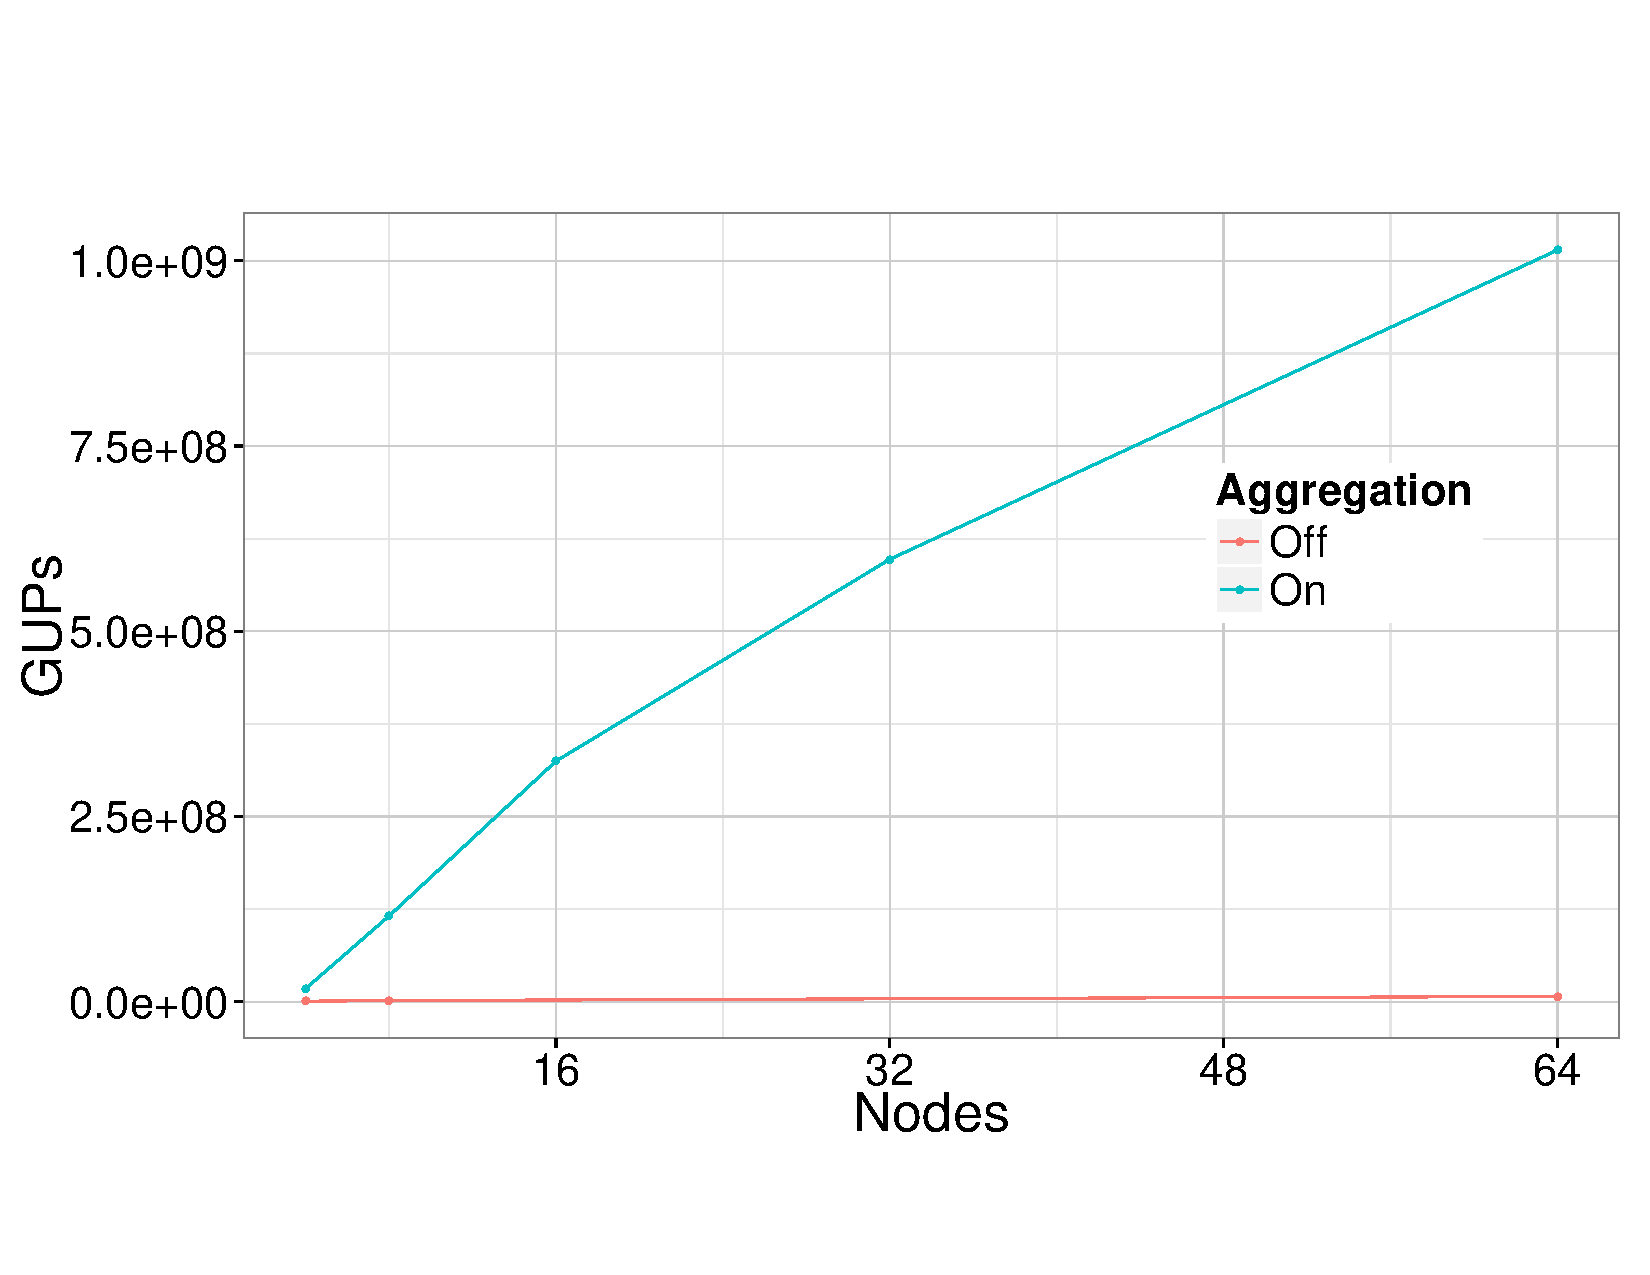
\includegraphics[width=0.5\textwidth]{results/gups/gups.pdf}
    \end{center}
    \caption{GUPS (giga updates per second) for \Grappa as the number of nodes grows.}
    \label{fig:grappa-gups}
\end{figure}

\paragraph{Putting it all together with Unbalanced Tree Search in
    memory (UTS).}
We now show the overall performance of \Grappa running UTS.
Figure~\ref{fig:grappa-uts}. The point of this experiment is to
demonstrate whether \Grappa's context switching and communication layers can in fact
be used together, while balancing workload, to run an irregular application efficiently. 
We look at two classes of trees, T1x and T3x, from the
original benchmark. T1x trees are very shallow and wide, while T3x
trees are very deep. When the access to each vertex is a random
access, the critical path to search T3x trees is very long. On such
trees, we do not expect there to be sufficient concurrency for any
system, including \Grappa, to achieve high throughput. \TODO{plot it
    if time}. To verify this, at the 16-node data point, the average active tasks per
core over the search is 775 and 13 for T1XL and T3L, respectively.

\begin{figure}[ht]
    \begin{center}
      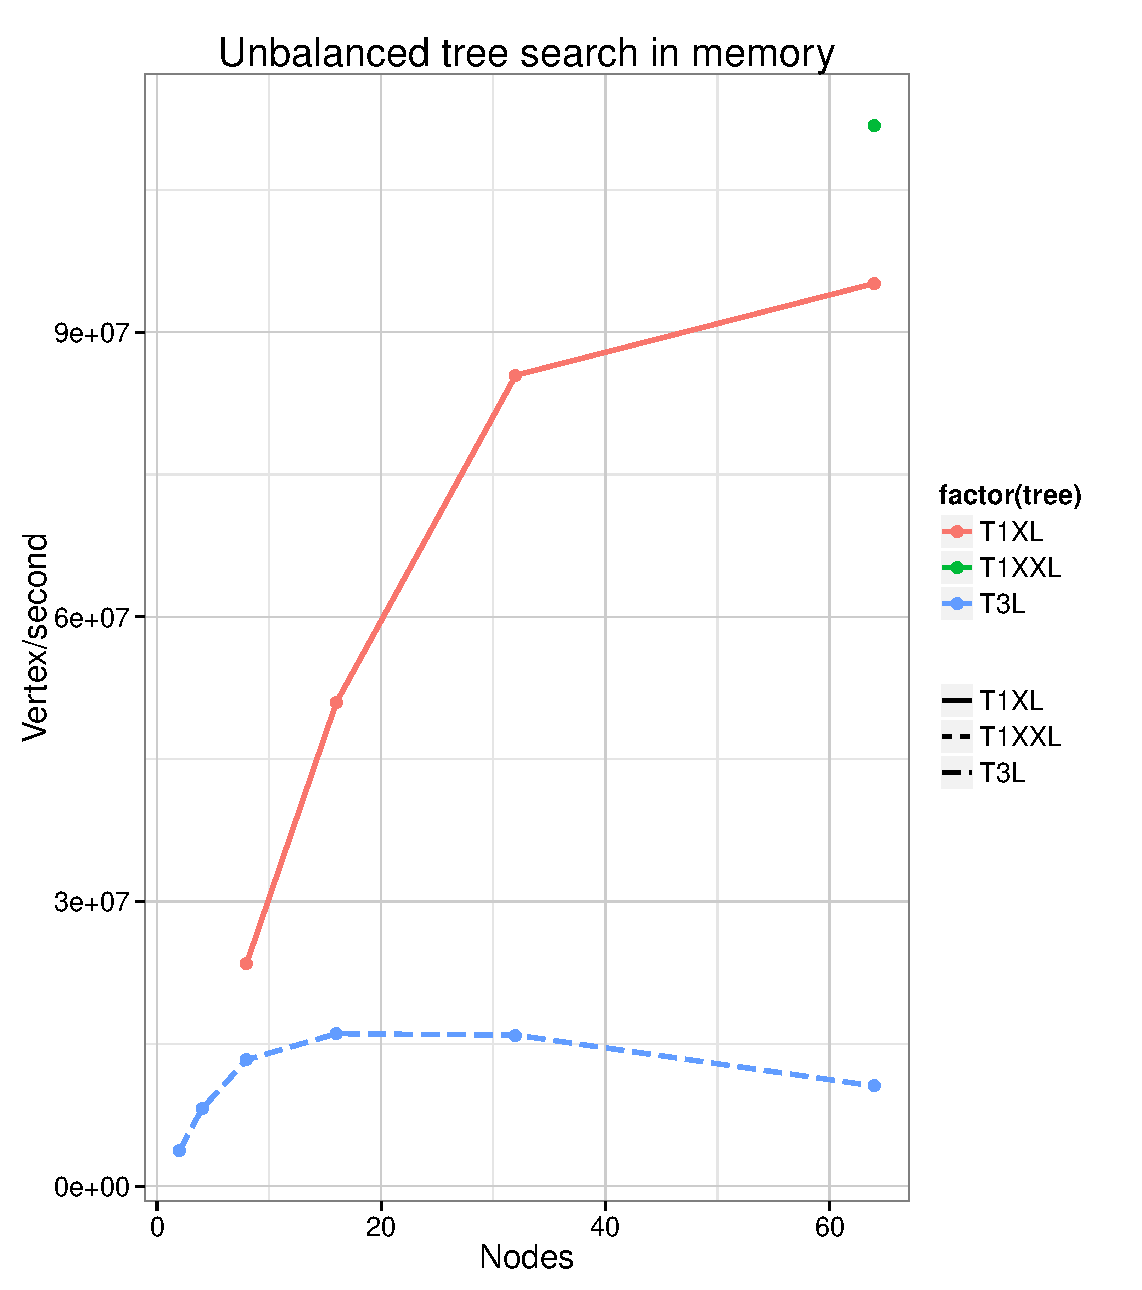
\includegraphics[width=0.5\textwidth]{figs/uts_scale.pdf}
    \end{center}
    \caption{Vertices per second in UTS on \Grappa as the number of nodes grows.}
    \label{fig:grappa-uts}
\end{figure}


\subsection{Comparing \Grappa to Other Systems}

In order to put \Grappa's performance into a general context, we compare it
with XMT running BFS, PageRank, IntSort, GUPS and UTS. Since XMT is a
different hardware platform, we also compare \Grappa with hand-tuned MPI
versions of BFS and GUPS running on the same hardware. Finally, we also
compare it with UTS written for UPC. We run all experiments with 64 nodes.

\begin{figure}[ht]
    \begin{center}
      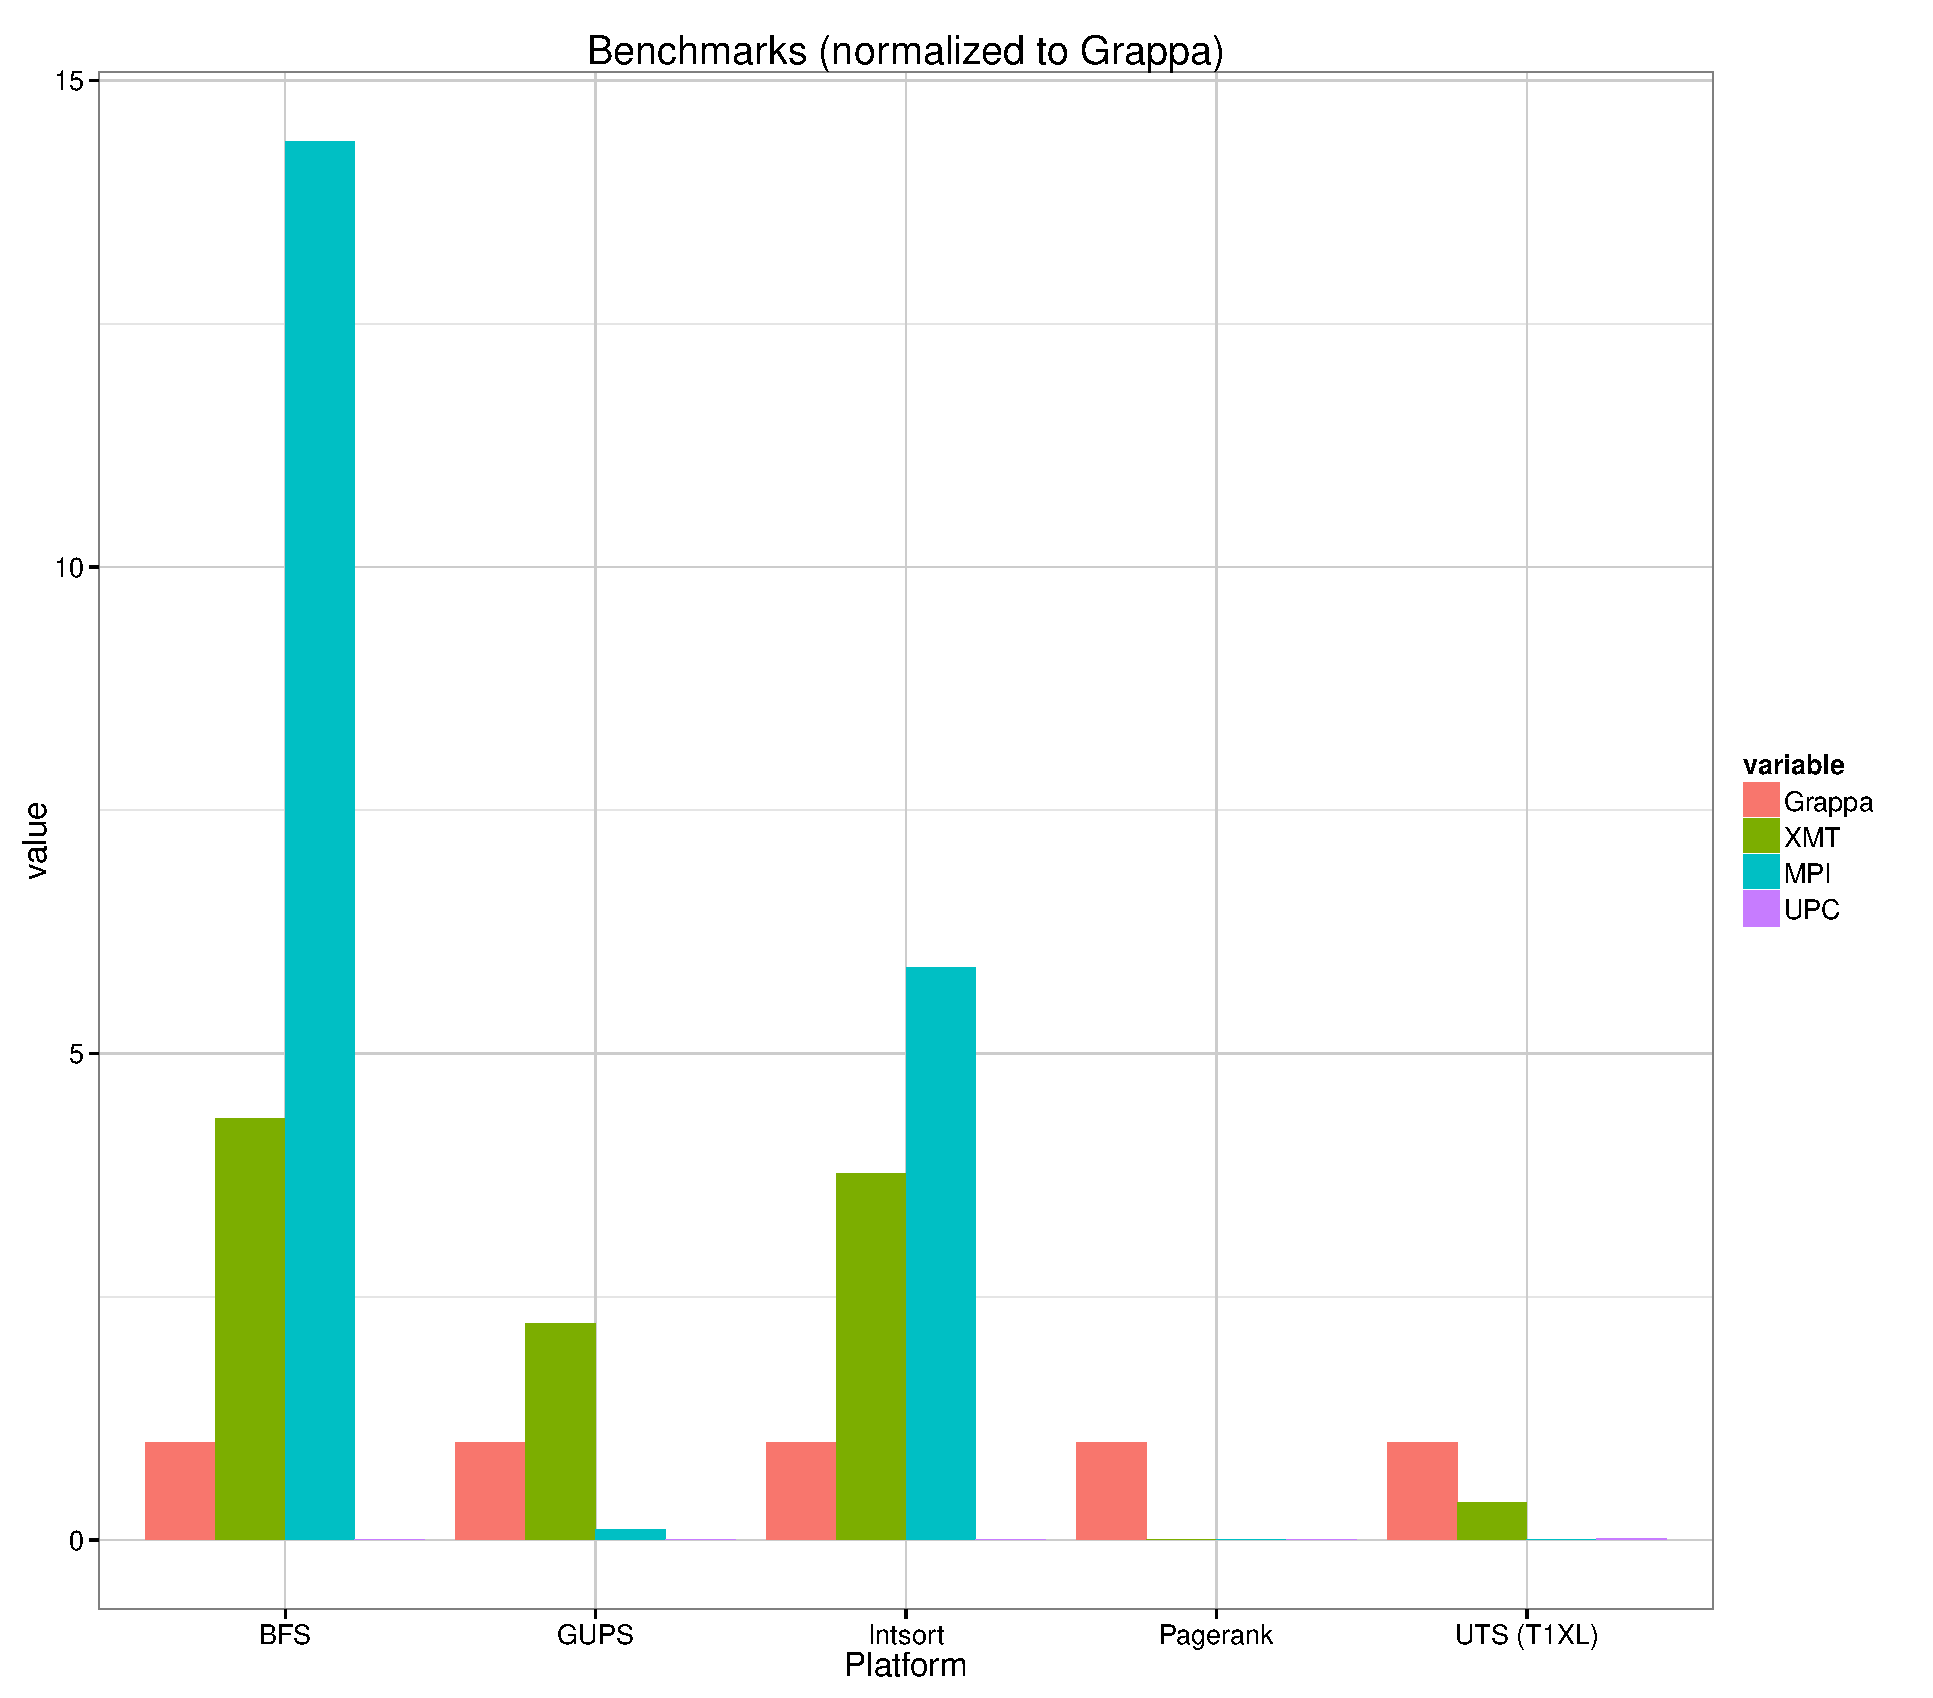
\includegraphics[width=0.5\textwidth]{results/benchmarks.pdf}
    \end{center}
    \caption{Comparing \Grappa with XMT, hand-tuned MPI and UPC.}
%bar chart, one set of bars per benchmark, one bar per system. runtime normalized to grappa.
    \label{fig:grappa-comparisons}
\end{figure}

Figure~\ref{fig:grappa-comparisons} shows the results. Overall, \Grappa is
within striking distance of XMT and UPC performance. However, it underperforms
compared to hand-tuned MPI. Nevertheless, this comparison needs to be taken
with a grain of salt for several reasons. First, we have not spent as much
time tuning \Grappa's implementations. This is supported by inspecting the BFS
MPI implementation we used, which clearly shows that it employs a lot of
algorithmic-specific optimizations. In fact, some of these optimizations
resemble some of what \Grappa does automatically, like message aggregation.
Second, the GUPS results presented earlier suggests that \Grappa performance
can do a lot better. \TODO{update this once we have more results. }

\subsection{Characterization}

\paragraph{Where execution time goes.}


\begin{figure}[ht]
    \begin{center}
      \begin{tabular}{c|c c c c}
        Benchmark     & Comm & User & Idle & Sched \\ \hline
        GUPS          & 6.60  & 42.94   & 47.74 & 2.80 \\
        BFS           & 54.84 & 30.90   & 10.94 & 3.43 \\ 
        Intsort       & 34.28 & 42.00   & 21.31 & 2.47 \\ 
        UTS           & 40.57 & 56.52   &  1.21 & 1.73 \\
        Pagerank      & 76.79 & 20.71   &  0.06 & 2.50 \\
      \end{tabular}
    \end{center}
    \caption{\Grappa\ execution time profile, in percent.}
%bar chart, one set of bars per benchmark, one bar per system. runtime normalized to grappa.
    \label{fig:grappa-profile}
\end{figure}

\TODO{PAGERANK:
    Without parallelizing the dot product, \Grappa cannot achieve
high utilization of workers proportional to the size of the data set.
Also mention that the cost of this is contention at the target
elements of vector.  The other parts of pagerank are super fast
(table?)
}

\paragraph{Message size and latency.}
Distribution if possible. With and without aggregation. 

\begin{figure}[ht]
    \begin{center}
      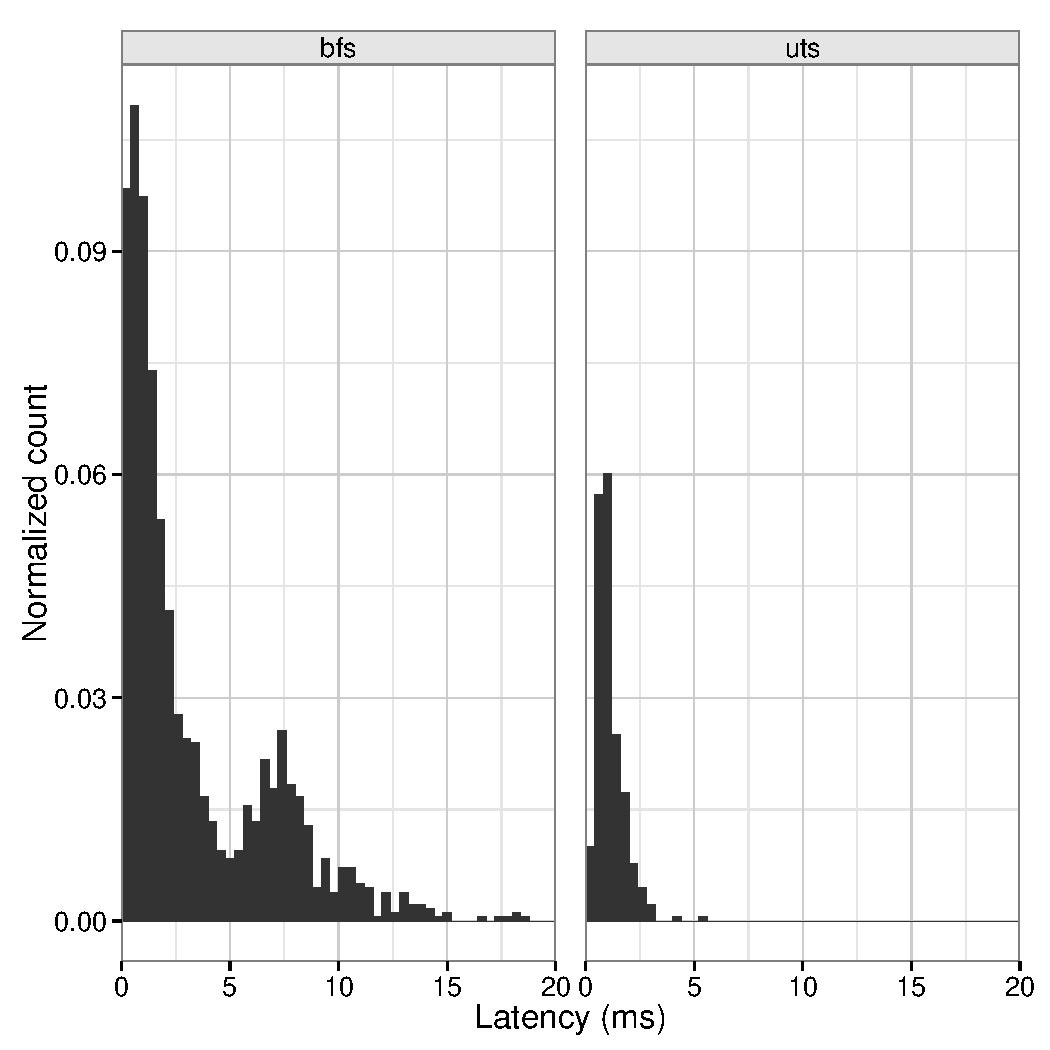
\includegraphics[width=0.5\textwidth]{results/histograms/latency_cmb.pdf}
    \end{center}
    \caption{Round-trip latency of delegate operations.}
%bar chart, one set of bars per benchmark, one bar per system. runtime normalized to grappa.
    \label{fig:grappa-latency}
\end{figure}

\begin{figure}[ht]
    \begin{center}
      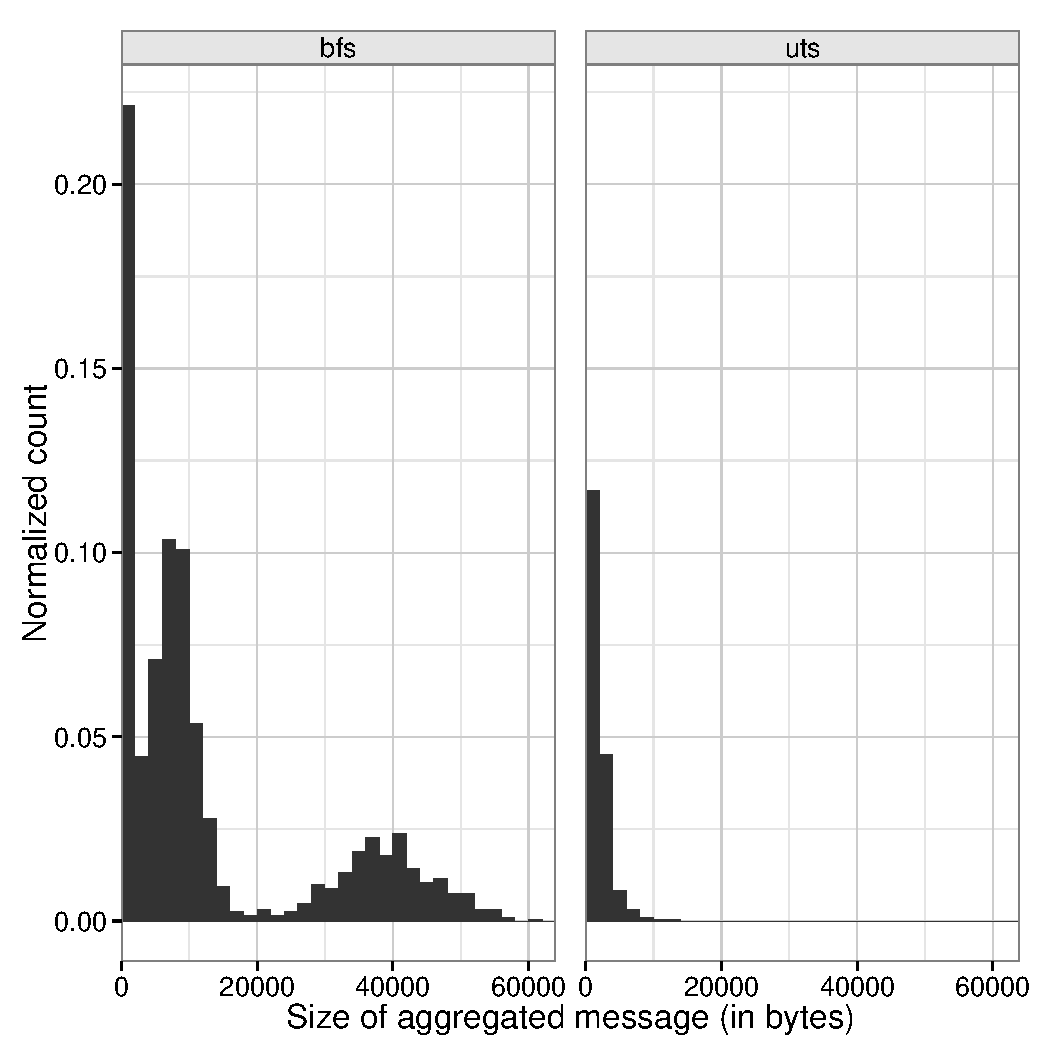
\includegraphics[width=0.5\textwidth]{results/histograms/rdma_bytes_sent_histogram_cmb.pdf}
    \end{center}
    \caption{Distribution of aggregated message sizes.}
%bar chart, one set of bars per benchmark, one bar per system. runtime normalized to grappa.
    \label{fig:grappa-message-size}
\end{figure}


\paragraph{Frequency of remote requests.}

\paragraph{Work stealing behavior.}
Performance loss of not having stealing. Ratio of \# of steals over total \# of task spawns. UTS needs stealing to work. 
















%%%%%%%%%%%%%%%%%%%%%%%%%%%%%%%%%%%%%% OLD %%%%%%%%%%%%%%%%%%

\comment{


Our evaluation begins with presentation of microbenchmark results, establishing
the intrinsic potential of \Grappa to provide random access bandwidth and latency tolerance. 
Next, we present application results, both for \Grappa and for other paradigms, as well
as comparing against the Cray XMT.  Finally, we present the impact of increased aggregation delay
on \Grappa results, thus exploring robustness to network scale.

\subsection{Microbenchmark Results}

\subsubsection{Random Access}
\TODO{Random access feed forward results on \Grappa.  optional: Results we measured for XMT.  Cite MPI results}
\subsubsection{Latency Tolerance}
\TODO{Simple ping test results -- eg, MPI ping, not the full blown aggregation ping test.  Random access blocking results on \Grappa.}
\subsubsection{Scheduling and Robustness}

\begin{figure}[ht]
    \begin{center}
      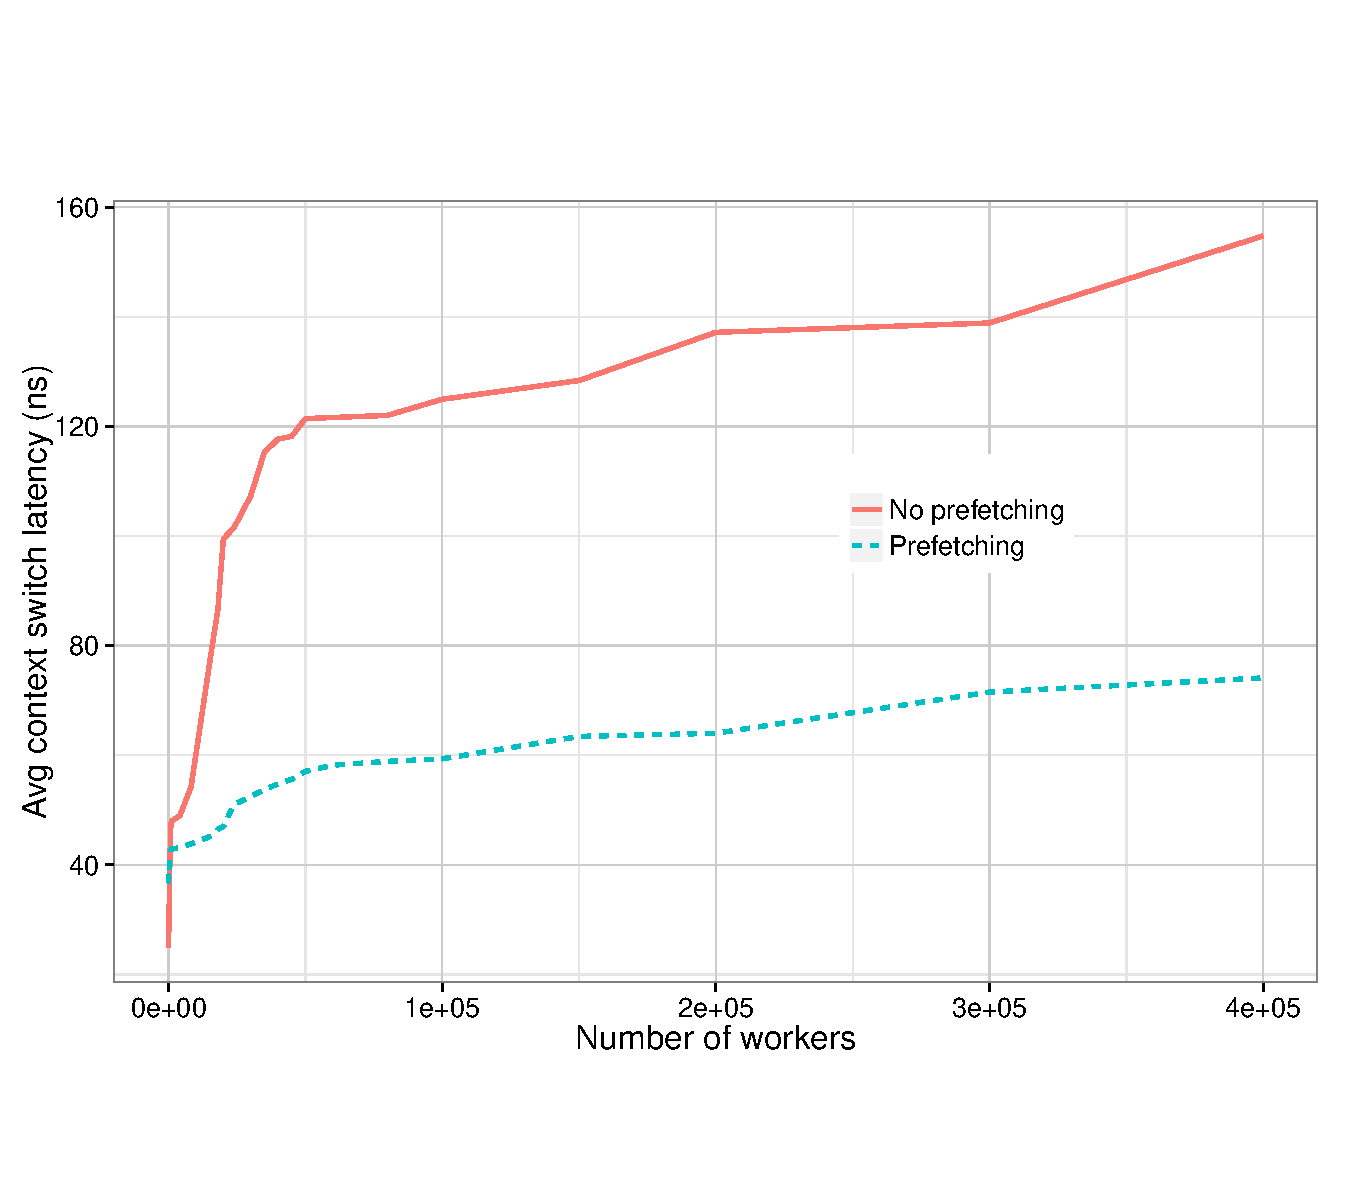
\includegraphics[width=0.5\textwidth]{figs/context_switch_time.pdf}
    \end{center}
    \caption{Average context switch time with 1 and 6 active cores,
        with and without prefetching.}
    \label{fig:context-switch-time}
\end{figure}

\begin{figure}[ht]
    \begin{center}
      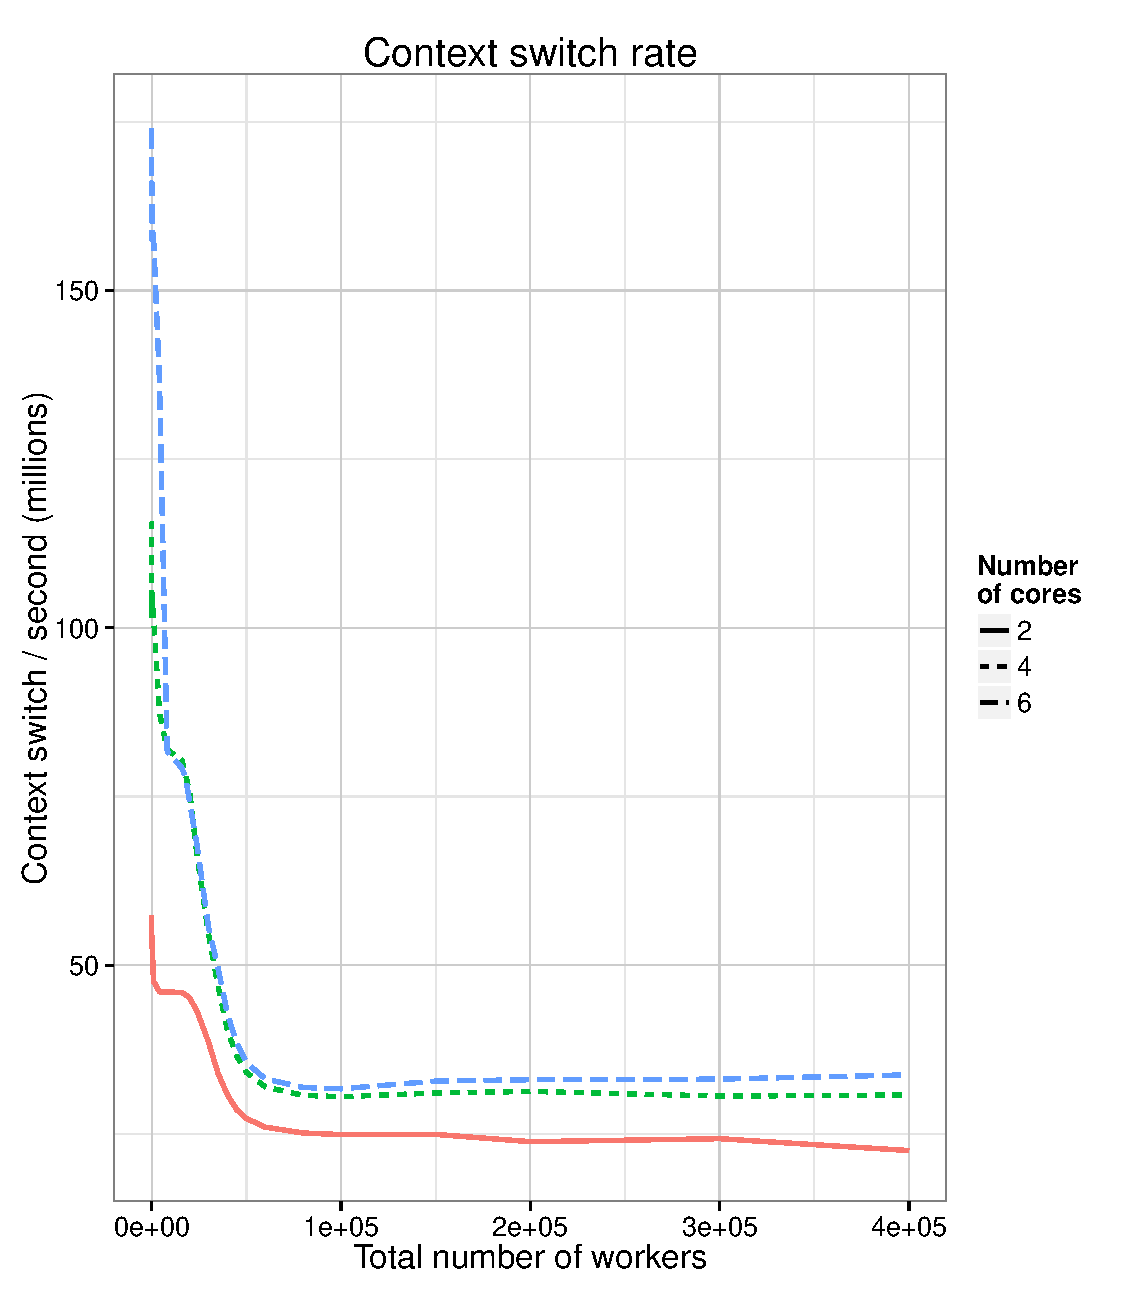
\includegraphics[width=0.5\textwidth]{figs/context_switch_bw.pdf}
    \end{center}
    \caption{Context switch rate with prefetching. Once the total
        size of contexts sufficiently exceeds last-level cache, most
    prefetches go to main memory and the rate becomes limited to the
    off-chip bandwidth.}
    \label{fig:context-switch-time}
\end{figure}

\TODO{Summary of what to write please expand: Reference above plots. Bandwidth of single socket is
    270Mcacheline/s. Each context is 4 cachelines: 1 for worker struct
    and 3 stack cachelines. We must read and write every context, so 8
    cacheline transfers per context switch. This asymptotically
    approaches 33.75Mcontexts/s as you increase the number of contexts
    (fewer and fewer in L3). Note that only 4+ cores reaches full rate
    because these westmere chips are balanced to not achieve full off-chip bandwidth until 4
    cores--bdmyers}

\TODO{Yield test results:  latency \& bandwidth.  Discussion of implications of zillions of contexts on robustness of latency tolerance preshadowing ~\ref{sec:scaling}}

\subsection{Application Results}
To evaluate \Grappa's performance with respect to the XMT, we ran each
of our three benchmarks on up to 16 nodes of each machine. \Grappa used
6 cores per node, with the best parameters chosen for each point. In
some cases, the XMT could not run the benchmark with 2 nodes, so the
point is omitted. \TODO{rewrite this!}
\subsubsection{Unbalanced Tree Search}\TODO{rewrite with new results}
%% UTS: performance comparison
\begin{figure}[ht]
    \begin{center}
      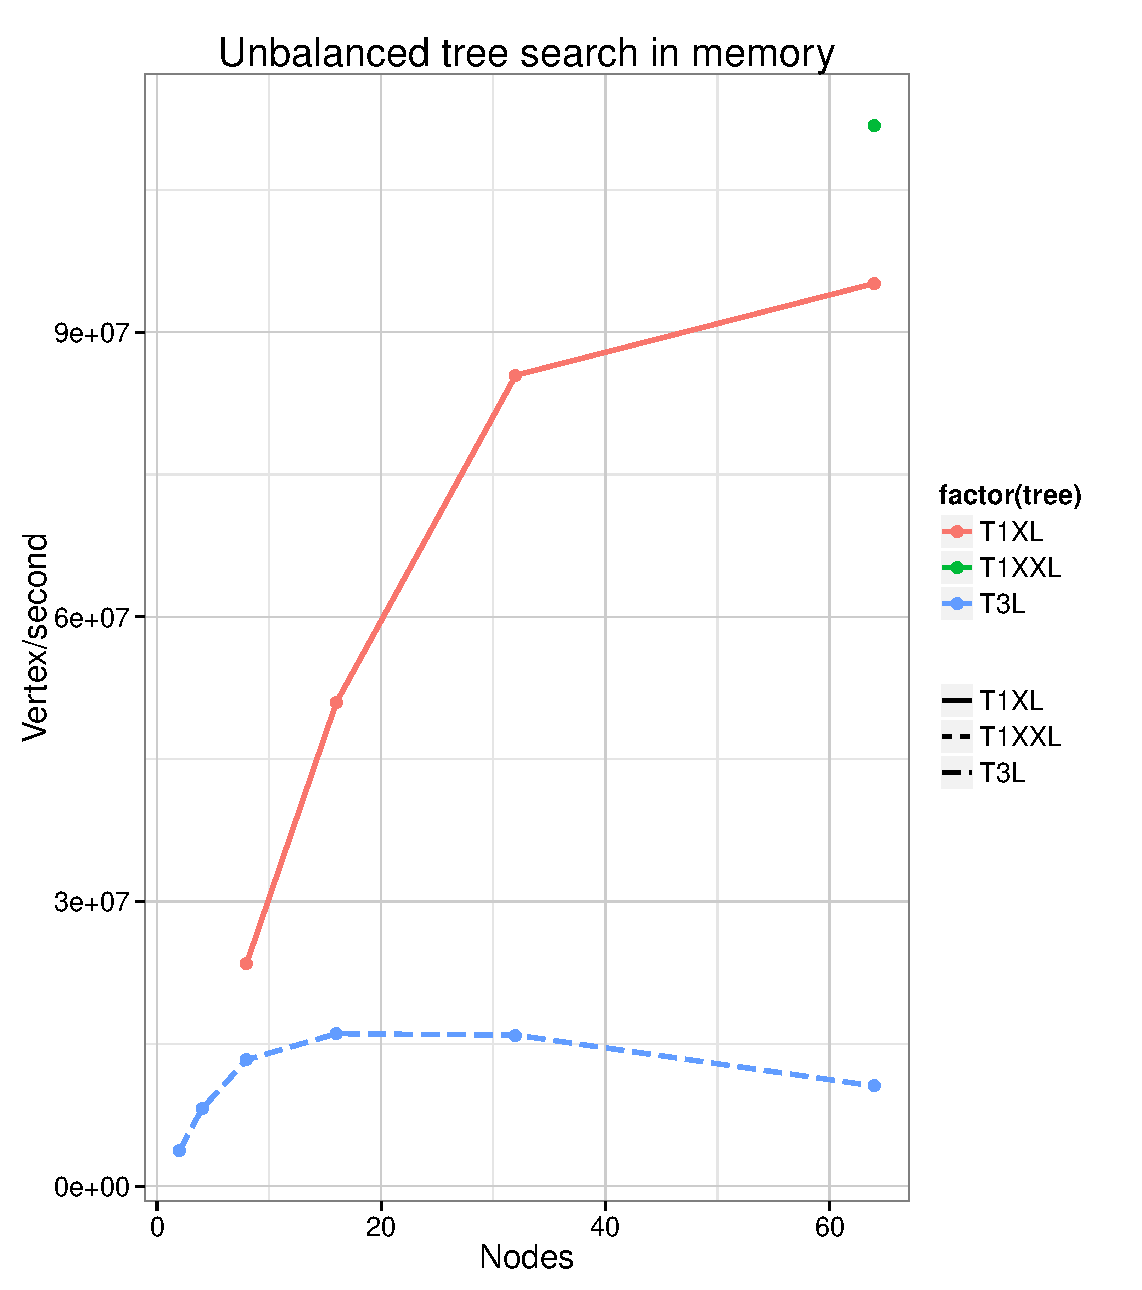
\includegraphics[width=0.5\textwidth]{figs/uts_scale.pdf}
    \end{center}
    \caption{Performance of in-memory unbalanced tree search.}
    \label{fig:uts_compare}
\end{figure}

We ran UTS-mem with a geometric 100M-vertex tree
(T1L). Figure~\ref{fig:uts_compare} shows the performance in terms of
number of vertices visited per second versus number of compute
nodes. \Grappa is 3.2 times faster than the XMT at 16 nodes.  As we will show later, the performance advantage \Grappa has over XMT increases as more nodes are added.  The main reason \Grappa performs better is the software-based delegate synchronization obviates the need for the retry-based synchronization that XMT uses.

\subsubsection{Breadth First Search}\TODO{rewrite with new results}
\begin{figure}[tH]
\begin{center}
  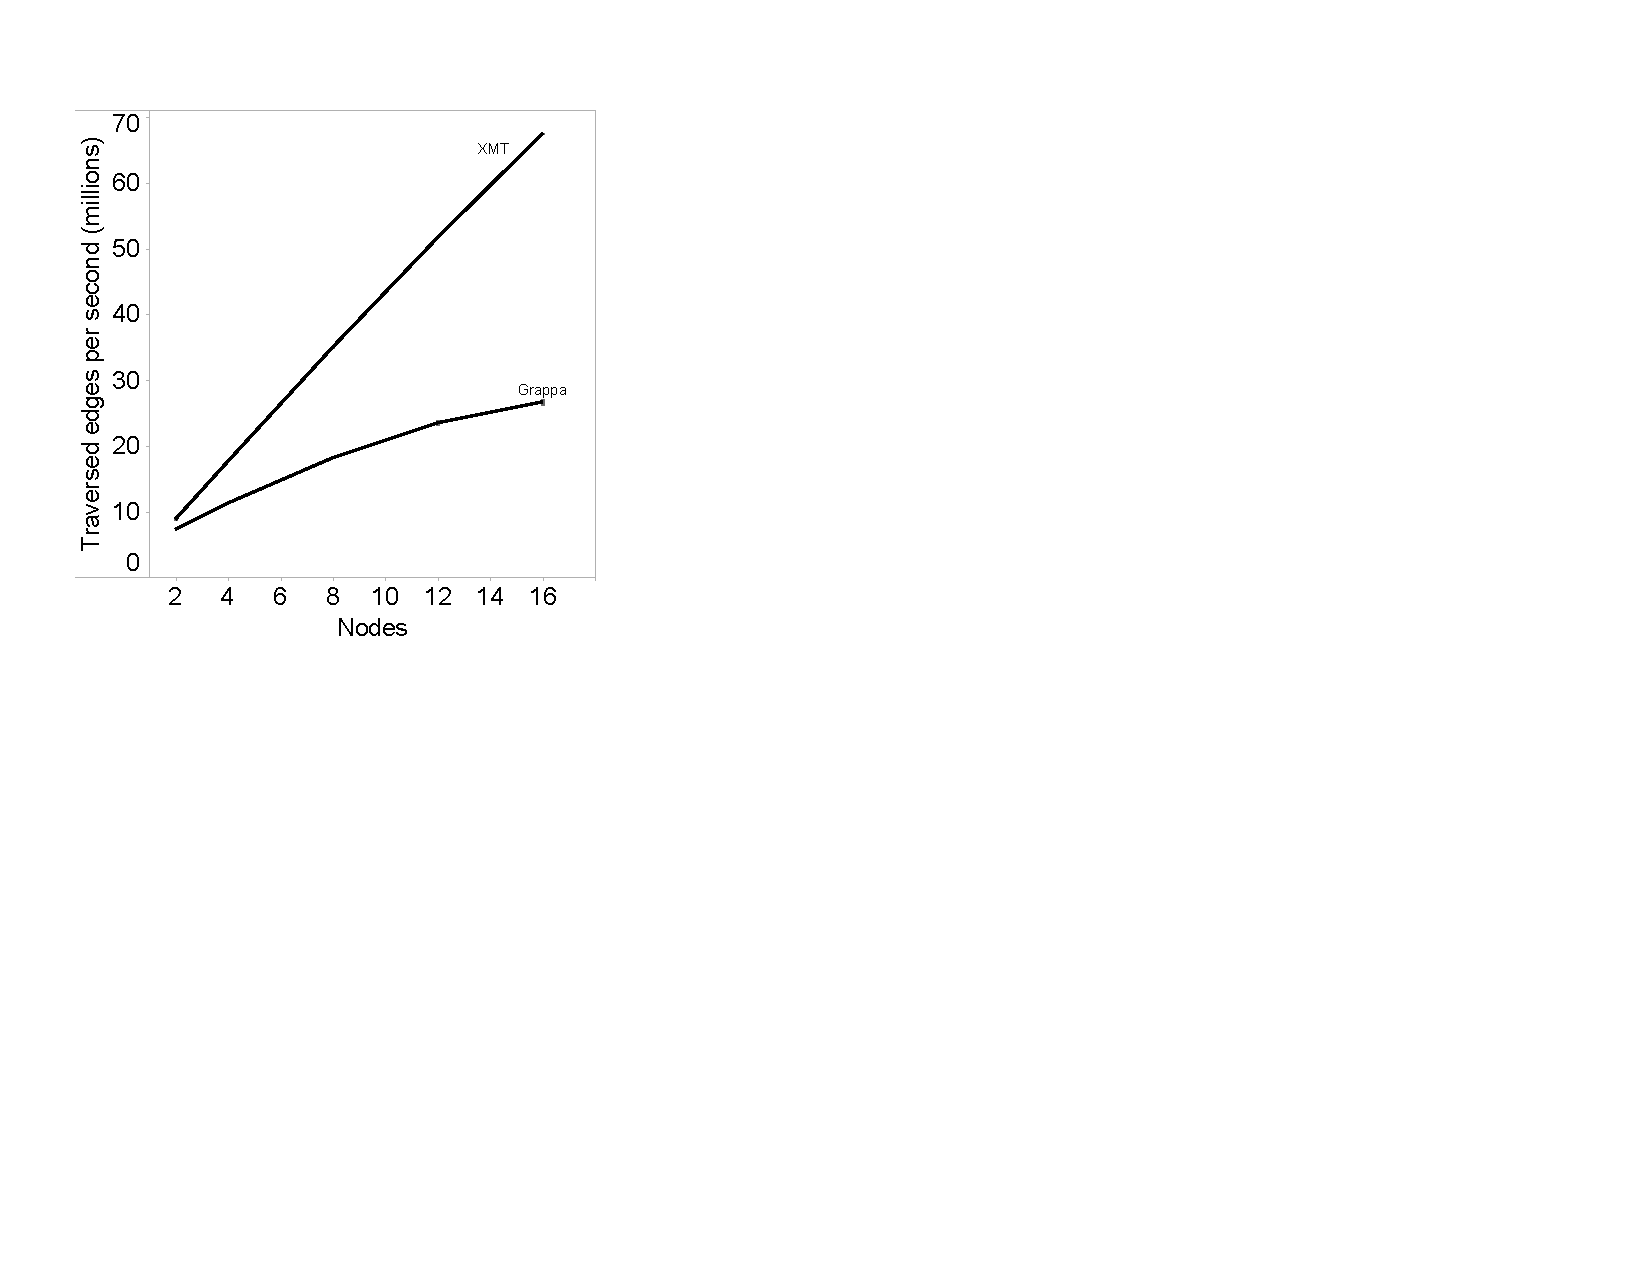
\includegraphics[width=0.95\columnwidth]{figs/bfs_performance}
\begin{minipage}{0.95\columnwidth}
  \caption{\label{fig:bfs-performance} BFS performance}
\end{minipage}
\vspace{-3ex}
\end{center}
\end{figure}

We ran BFS on a synthetic Kronecker graph with $2^{25}$ vertices and
$2^{29}$ edges (25 GB of data). Figure~\ref{fig:bfs-performance} shows
our performance in terms of graph edges traversed per second. The XMT
is 2.5 times faster than \Grappa at 16 nodes.  Performance does scale at a constant rate for \Grappa, suggesting that adding more nodes will increase performance.

\subsubsection{Approximate Betweenness Centrality}\TODO{rewrite with new results}
\begin{figure}[tH]
\begin{center}
  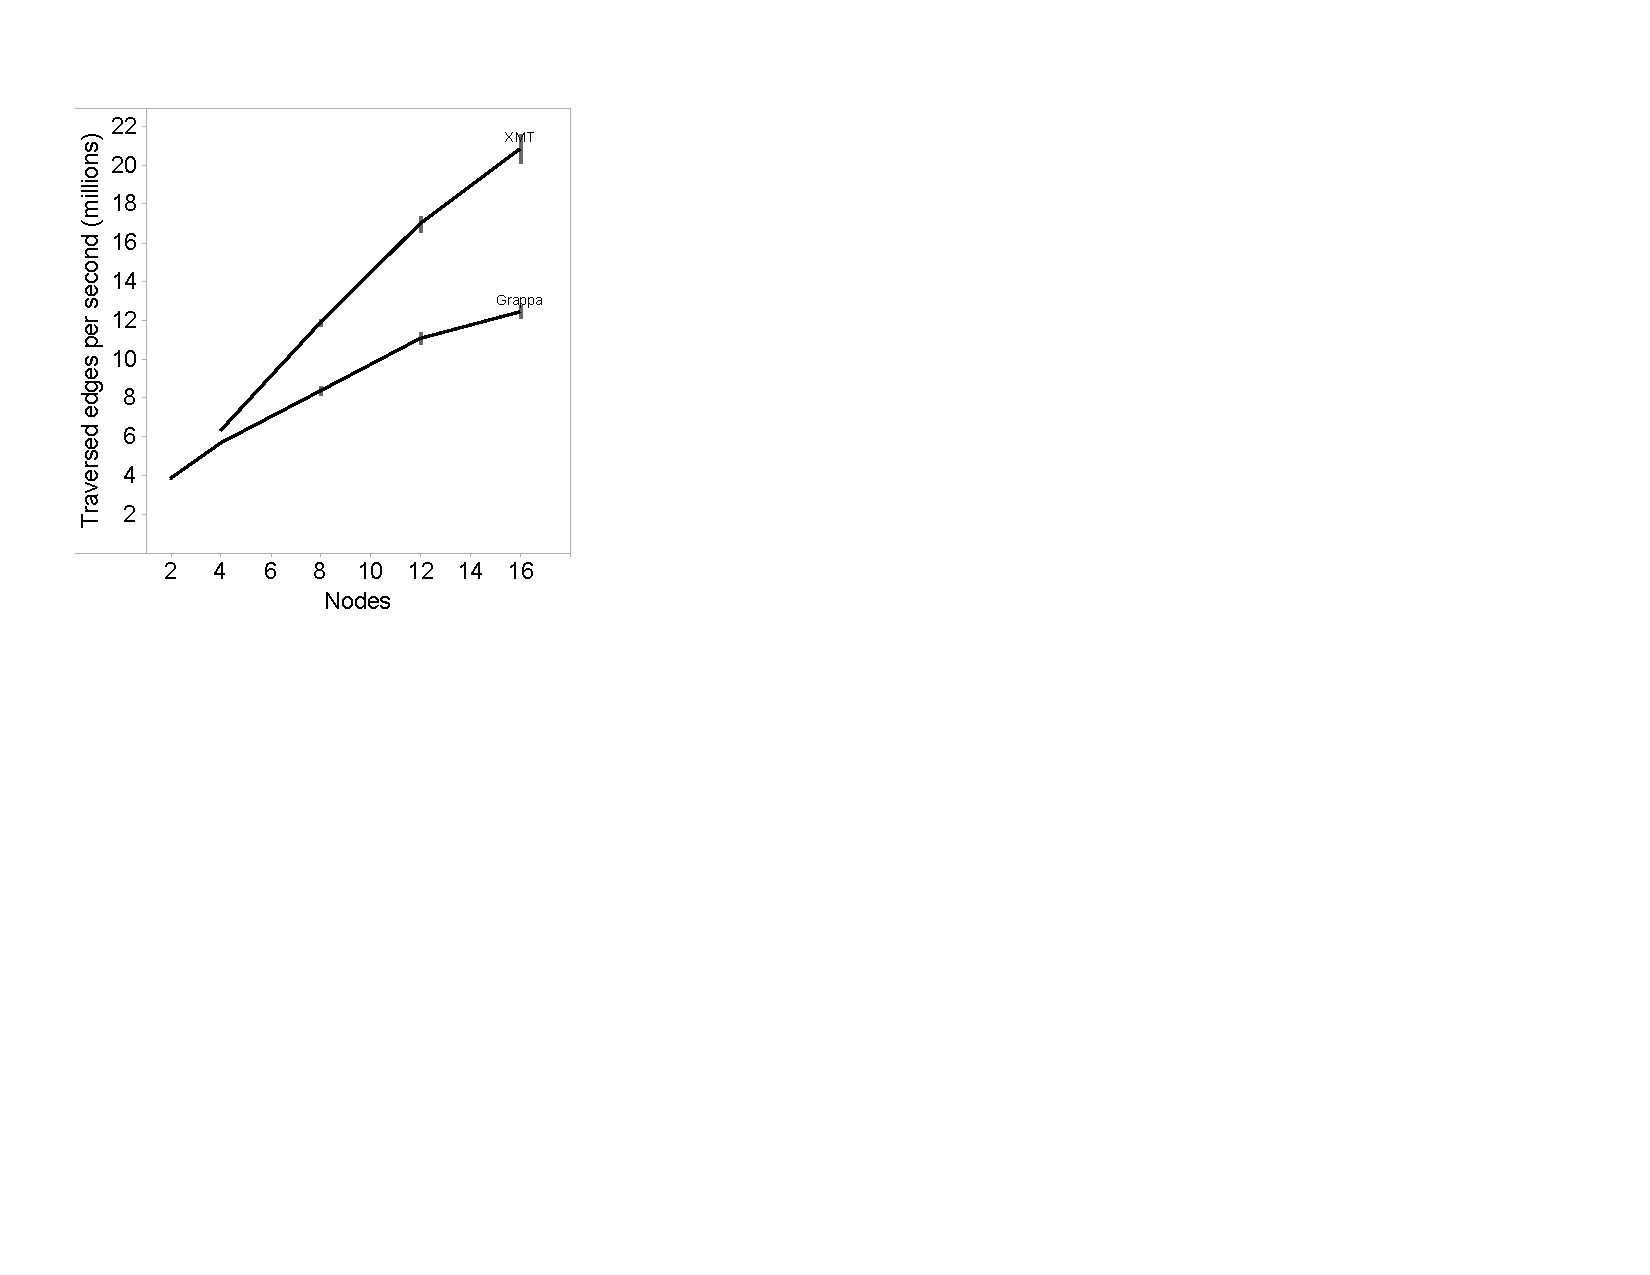
\includegraphics[width=0.95\columnwidth]{figs/centrality_performance}
\begin{minipage}{0.95\columnwidth}
  \caption{\label{fig:centrality-performance} Centrality performance}
\end{minipage}
\vspace{-3ex}
\end{center}
\end{figure}

We ran Betweenness Centrality on the same scale 25 Kronecker graph as
we did for BFS. Figure~\ref{fig:centrality-performance} shows our
performance in terms of graph edges traversed per second. At 16 XMT
processors/cluster nodes, the XMT is 1.75 times faster than \Grappa.

% Got rid of this discussion of UTS by itself, tried to work the highlights in below
%\paragraph{UTS-Mem}
%We ran UTS-Mem on \Grappa and the XMT with a geometric 1.6B-vertex tree
%(T1XL) and a geometric 4.2B-vertex tree (T1XXL), using up to 128
%nodes---the maximum we had available for each. \Grappa results are for 5 cores per node. \Grappa with 20 machines is faster than the entire XMT of 128 processors.

%\Grappa achieves \checkme{188Mvert/s} with 128 nodes and the XMT
%achieves only 50Mvert/s, plateauing at 60 nodes. Beyond 90 nodes, \Grappa adds 1.4 Mvert/s/node.
%The XMT scales at 850 Kvert/s/node, until it plateaus. \Grappa keeps
%scaling up through 128 nodes, although scaling
%declines because of the unscalability of our aggregation mechanism as
%number of network endpoints increases. 
%
%Despite our efforts to tune the UTS implementation specific to the 
%XMT, performance does not scale well with increasing processor count,
%flattening out around 60 processors.  When we increase the size of
%the tree from 100M to 4.2B, we find that performance does not improve,
%suggesting that performance is not limited by task parallelism.
%Cray's performance tools show an increasing number of memory
%retry operations for failed synchronization operations generated by
%the runtime, which create network contention.
%
To determine how \Grappa's performance scales compared to the performance of the entire XMT, we ran a set of experiments up to all 128 XMT processors and 128 cluster nodes. For the XMT, the number of allowed processors was varied up to the entire machine, with some minor tuning of stream parameters needed to get optimal performance. For \Grappa, parameters such as cores per node, aggregator timeouts, and parallel threshold were tuned to get the best performance for each node count. All of the benchmarks continue to improve out to 128 nodes for \Grappa. UTS continues to fare better than the XMT with large node counts, with the XMT appearing to plateau at 60 processors due to contention from synchronization retries, while \Grappa handles this by suspending tasks until messages return. For BFS and Centrality, the XMT scales approximately a constant factor better than \Grappa. We attribute this to a limitation in the current aggregator design and network stack that \Grappa uses.  This limits the practical number of cores we can use to 6 per node (adding more cores per node \emph{decreases} performance).  Ironically, this limitation makes \Grappa applications compute-bound instead of network-bound.  Work is ongoing to rework the Infiniband driver stack and aggregation interface to remove this limitation and improve aggregation addressing using local routing.

\begin{figure}[ht]
    \begin{center}
      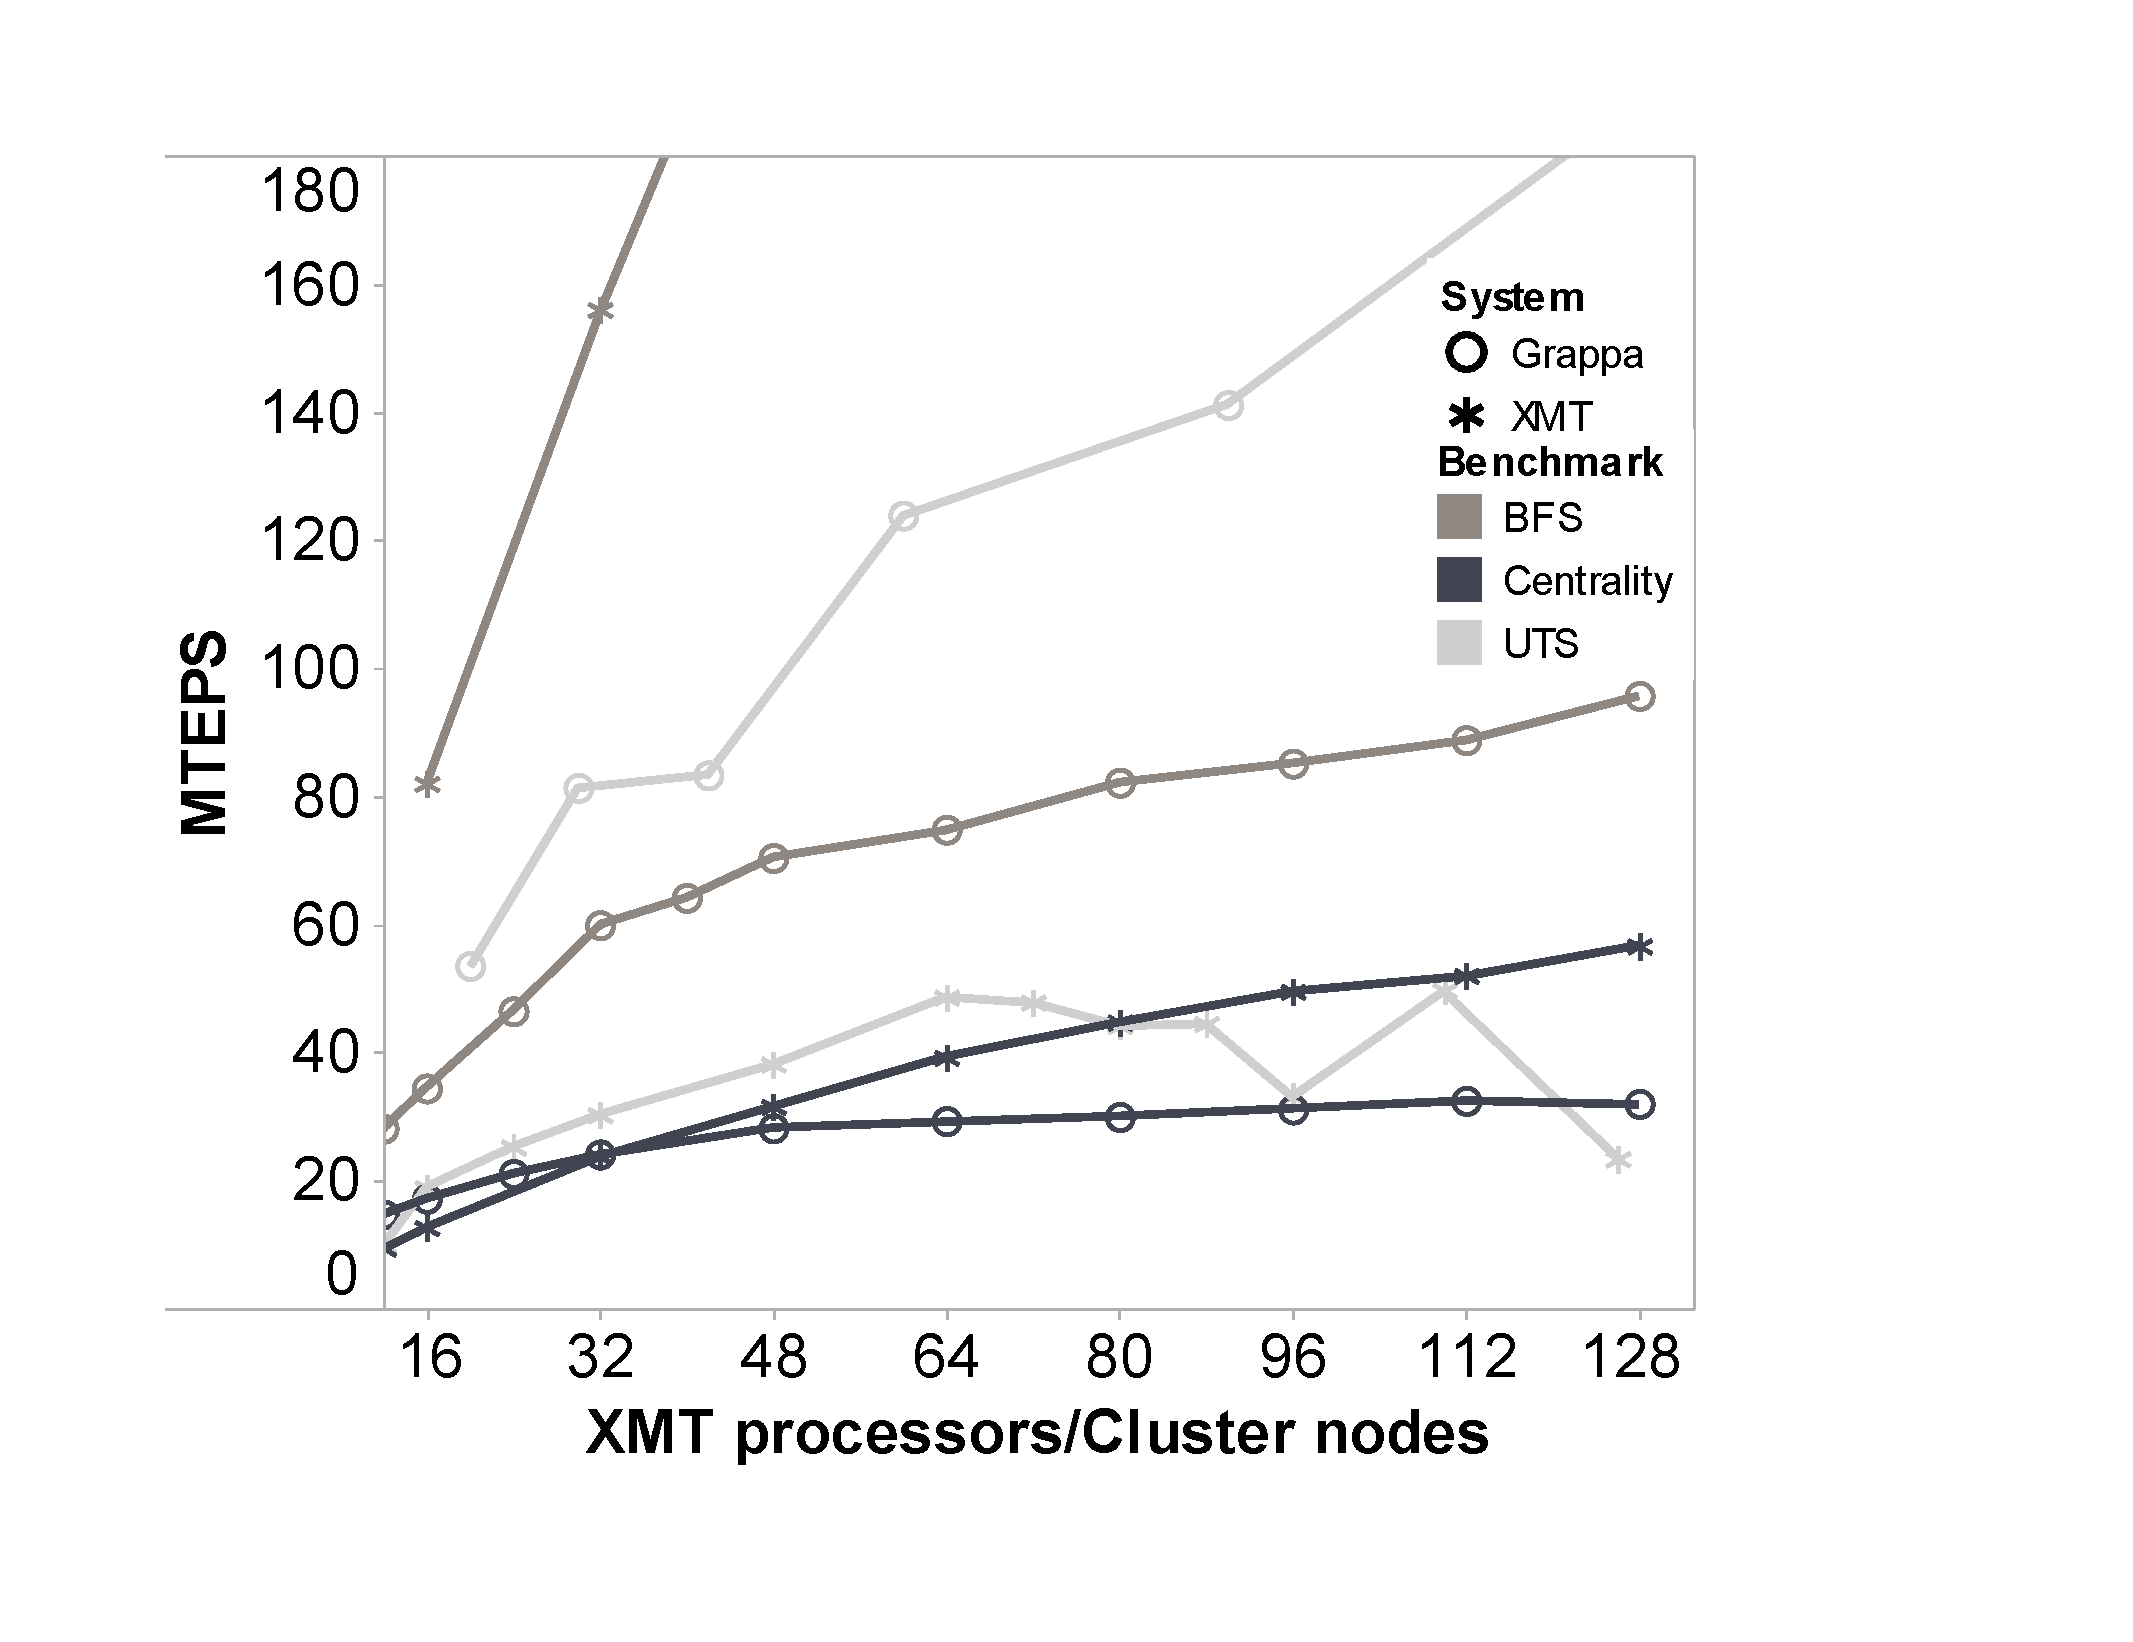
\includegraphics[width=0.5\textwidth]{figs/scaling_cropped.pdf}
    \end{center}
    \caption{Scaling number of nodes: \Grappa continues to perform significantly better than XMT for UTS but scales a constant factor slower than XMT for BFS (4x slower) and Centrality (2x slower). }
    \label{fig:uts_threshold}
\end{figure}

\subsection{Scaling}\label{sec:scaling} \TODO{rewrite with new results}

\subsubsection{Network Aggregation Performance and Robustness}

\begin{figure}[htb]
\begin{center}
  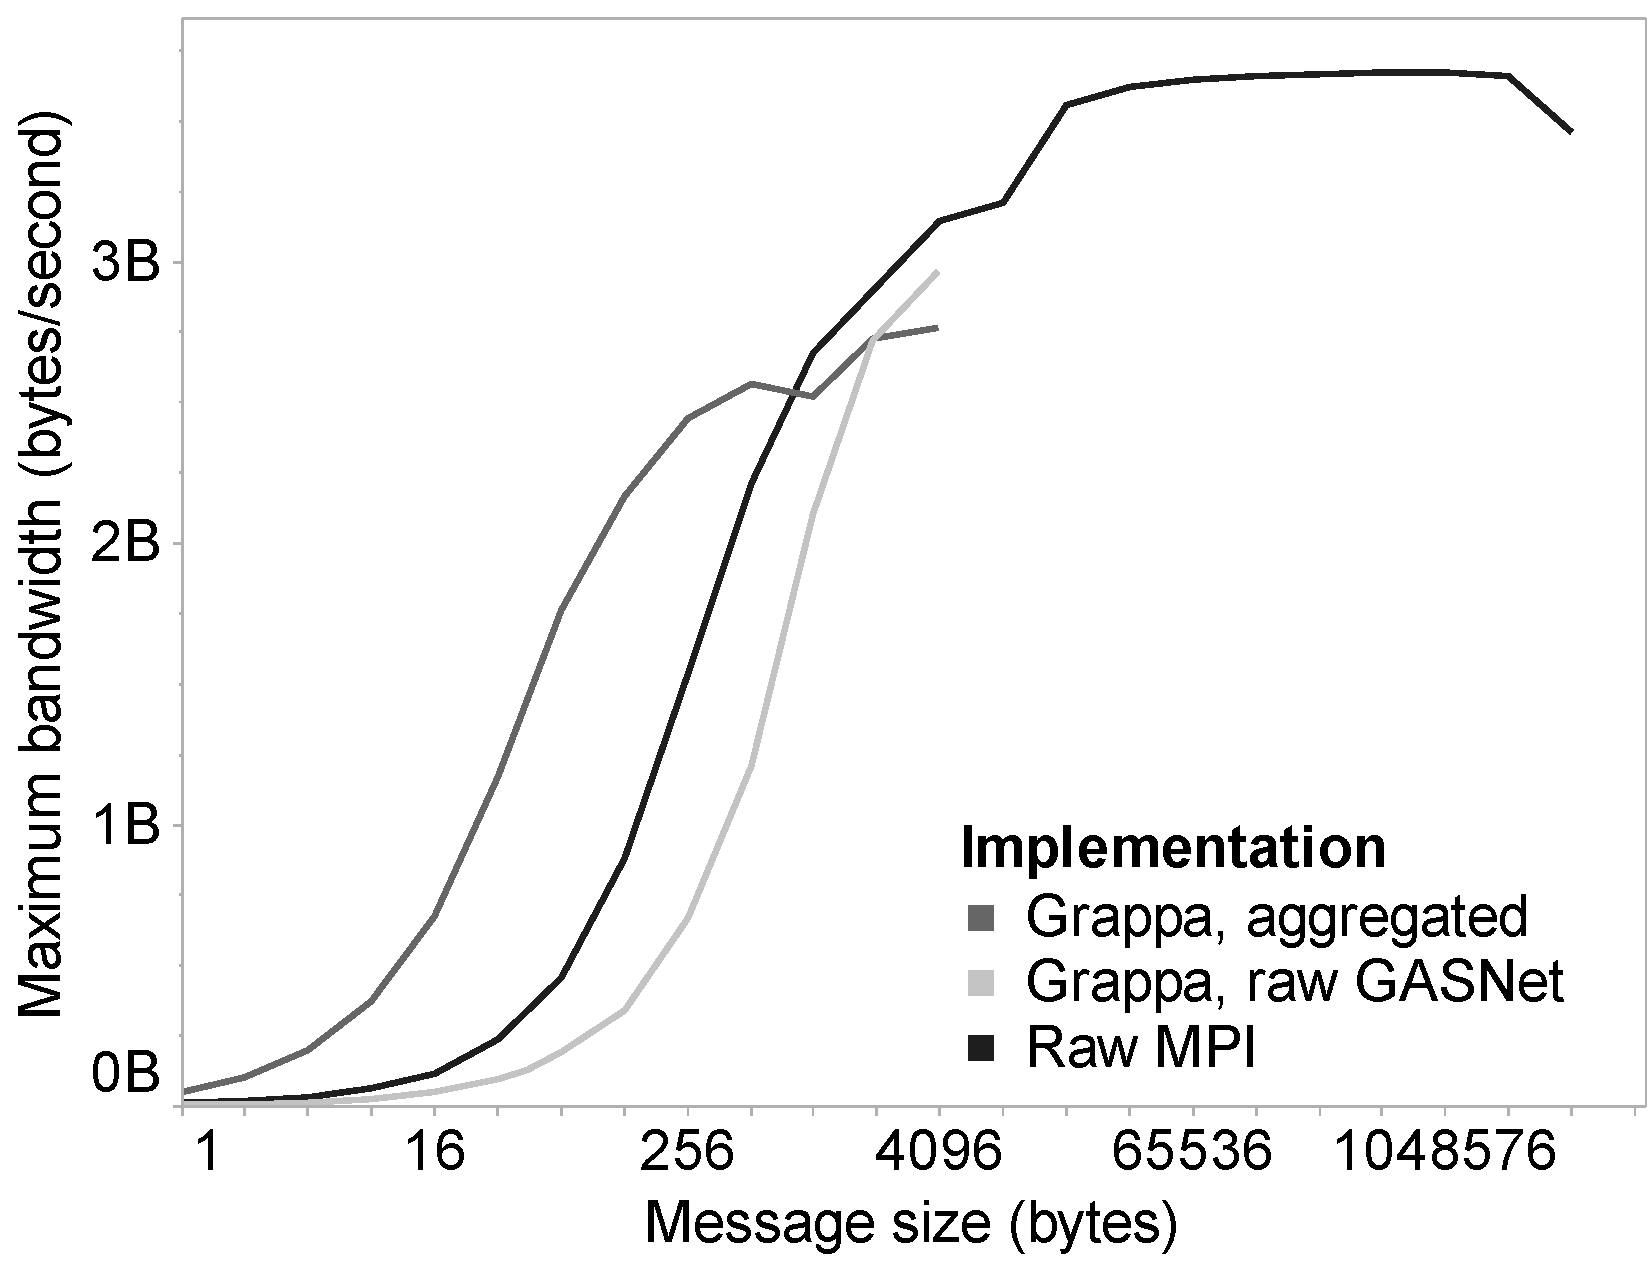
\includegraphics[width=0.95\columnwidth]{figs/aggregator_ping}
\begin{minipage}{0.95\columnwidth}
  \caption{\label{fig:aggregator-ping} Bandwidth versus message size
    unidirectional ping test for \Grappa with aggregation, \Grappa with
    raw GASNet messages, and MPI. Aggregation provides an 11x
    bandwidth benefit at our common operating point.}
\end{minipage}
\vspace{-3ex}
\end{center}
\end{figure}

To evaluate the benefits of network aggregation, we ran two experiments.
First, we ran a simple unidirectional ping test to see the maximum
benefit the aggregator can provide in terms of improved network
efficiency. Second, we ran BFS with the aggregator disabled in order to
measure its benefit on an application.

To implement the ping test, we wrote a simple \Grappa application where
the cores of one node send messages as fast as possible to the cores
of another node. We vary the size of the payload up the maximum
payload size supported by the aggregator (nearly 4KB). Each core has a
single task sending to a single destination, so this is a best case
scenario for the aggregator. To see the benefit of the aggregator, we
added a bypass that lets us send messages directly through GASNet. We
also compare against the OSU \texttt{osu\_mbw\_mr} benchmark
\cite{osu:mpi}  compiled against OpenMPI 1.5.3; this
benchmark has the same pattern of communication but doesn't have the
overhead of \Grappa's context switching.

The results are shown in Figure~\ref{fig:aggregator-ping}. There are
two key observations.

First, small message performance against the existing libraries is, as expected, poor. The MPI application test shows us that peak per node
bandwidth supported by our infiniband card is 3.4GB/s. This is
achievable only with large messages; we must send 16KB packets to get
within 5 percent of peak bandwidth. But in our benchmarks, we saw
average message between 32 and 64 bytes. At 32 bytes, the MPI test is
using less than 7 percent of its peak bandwidth. \Grappa sending
messages directly through GASNet uses less than 3 percent of the peak
bandwidth.

Second, aggregation has the potential to improve this situation by an
order of magnitude. With aggregation, \Grappa is able to send 32-byte
messages over 12 times faster than using GASNet directly. This is a
more respectable 32 percent of peak bandwidth. Due to expedient design
decisions, \Grappa's aggregator limits its aggregation to 4KB; this
limits its peak achievable bandwidth to 75 percent of the actual
peak.

This comparison is the best possible case for the aggregator. In
order to verify that the aggregator still has value on actual
applications at scale, we ran a small (100M node tree) UTS-Mem
with the aggregator disabled, on 16 nodes.
Figure~\ref{fig:no-aggregation-uts}. At this configuration, the aggregator
improves our application performance by 10x. 

\begin{figure}[htb]
\begin{center}
  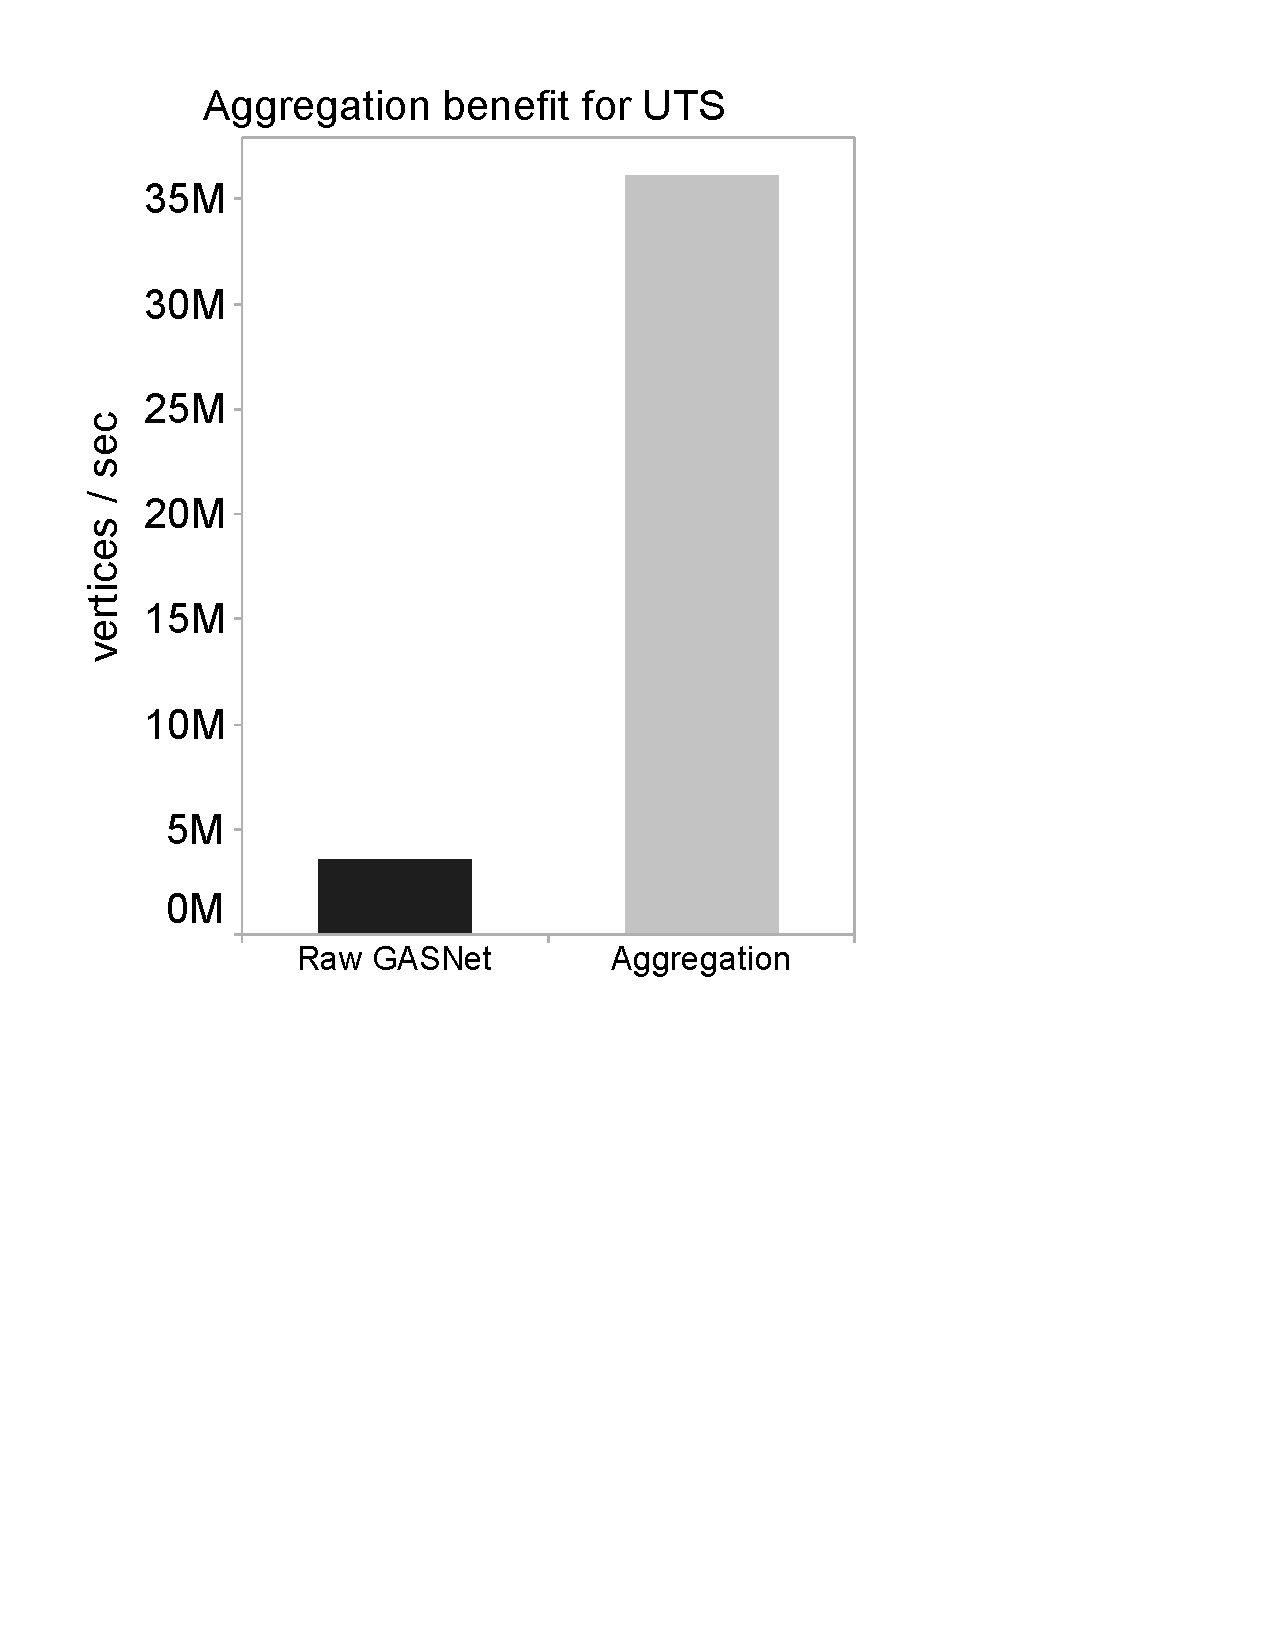
\includegraphics[width=0.95\columnwidth]{figs/no_aggregation_uts.pdf}
\begin{minipage}{0.95\columnwidth}
  \caption{\label{fig:no-aggregation-uts} Performance of UTS on 16
      nodes with and without \Grappa's aggregation.}
\end{minipage}
\vspace{-3ex}
\end{center}
\end{figure}

\subsection{Scaling}
% Got rid of this discussion of UTS by itself, tried to work the highlights in below
%\paragraph{UTS-Mem}
%We ran UTS-Mem on \Grappa and the XMT with a geometric 1.6B-vertex tree
%(T1XL) and a geometric 4.2B-vertex tree (T1XXL), using up to 128
%nodes---the maximum we had available for each. \Grappa results are for 5 cores per node. \Grappa with 20 machines is faster than the entire XMT of 128 processors.
%\Grappa achieves \checkme{188Mvert/s} with 128 nodes and the XMT
%achieves only 50Mvert/s, plateauing at 60 nodes. Beyond 90 nodes, \Grappa adds 1.4 Mvert/s/node.
%The XMT scales at 850 Kvert/s/node, until it plateaus. \Grappa keeps
%scaling up through 128 nodes, although scaling
%declines because of the unscalability of our aggregation mechanism as
%number of network endpoints increases. 
%
%Despite our efforts to tune the UTS implementation specific to the 
%XMT, performance does not scale well with increasing processor count,
%flattening out around 60 processors.  When we increase the size of
%the tree from 100M to 4.2B, we find that performance does not improve,
%suggesting that performance is not limited by task parallelism.
%Cray's performance tools show an increasing number of memory
%retry operations for failed synchronization operations generated by
%the runtime, which create network contention.
%
To determine how \Grappa's performance scales compared to the performance of the entire XMT, we ran a set of experiments up to all 128 XMT processors and 128 cluster nodes. For the XMT, the number of allowed processors was varied up to the entire machine, with some minor tuning of stream parameters needed to get optimal performance. For \Grappa, parameters such as cores per node, aggregator timeouts, and parallel threshold were tuned to get the best performance for each node count. All of the benchmarks continue to improve out to 128 nodes for \Grappa. UTS continues to fare better than the XMT with large node counts, with the XMT appearing to plateau at 60 processors due to contention from synchronization retries, while \Grappa handles this by suspending tasks until messages return. For BFS and Centrality, the XMT scales approximately a constant factor better than \Grappa. We attribute this to a limitation in the current aggregator design and network stack that \Grappa uses.  This limits the practical number of cores we can use to 6 per node (adding more cores per node \emph{decreases\/} performance).  Ironically, this limitation makes \Grappa applications compute-bound instead of network-bound.  Work is ongoing to rework the Infiniband driver stack and aggregation interface to remove this limitation and improve aggregation addressing using local routing.

\begin{figure}[ht]
    \begin{center}
      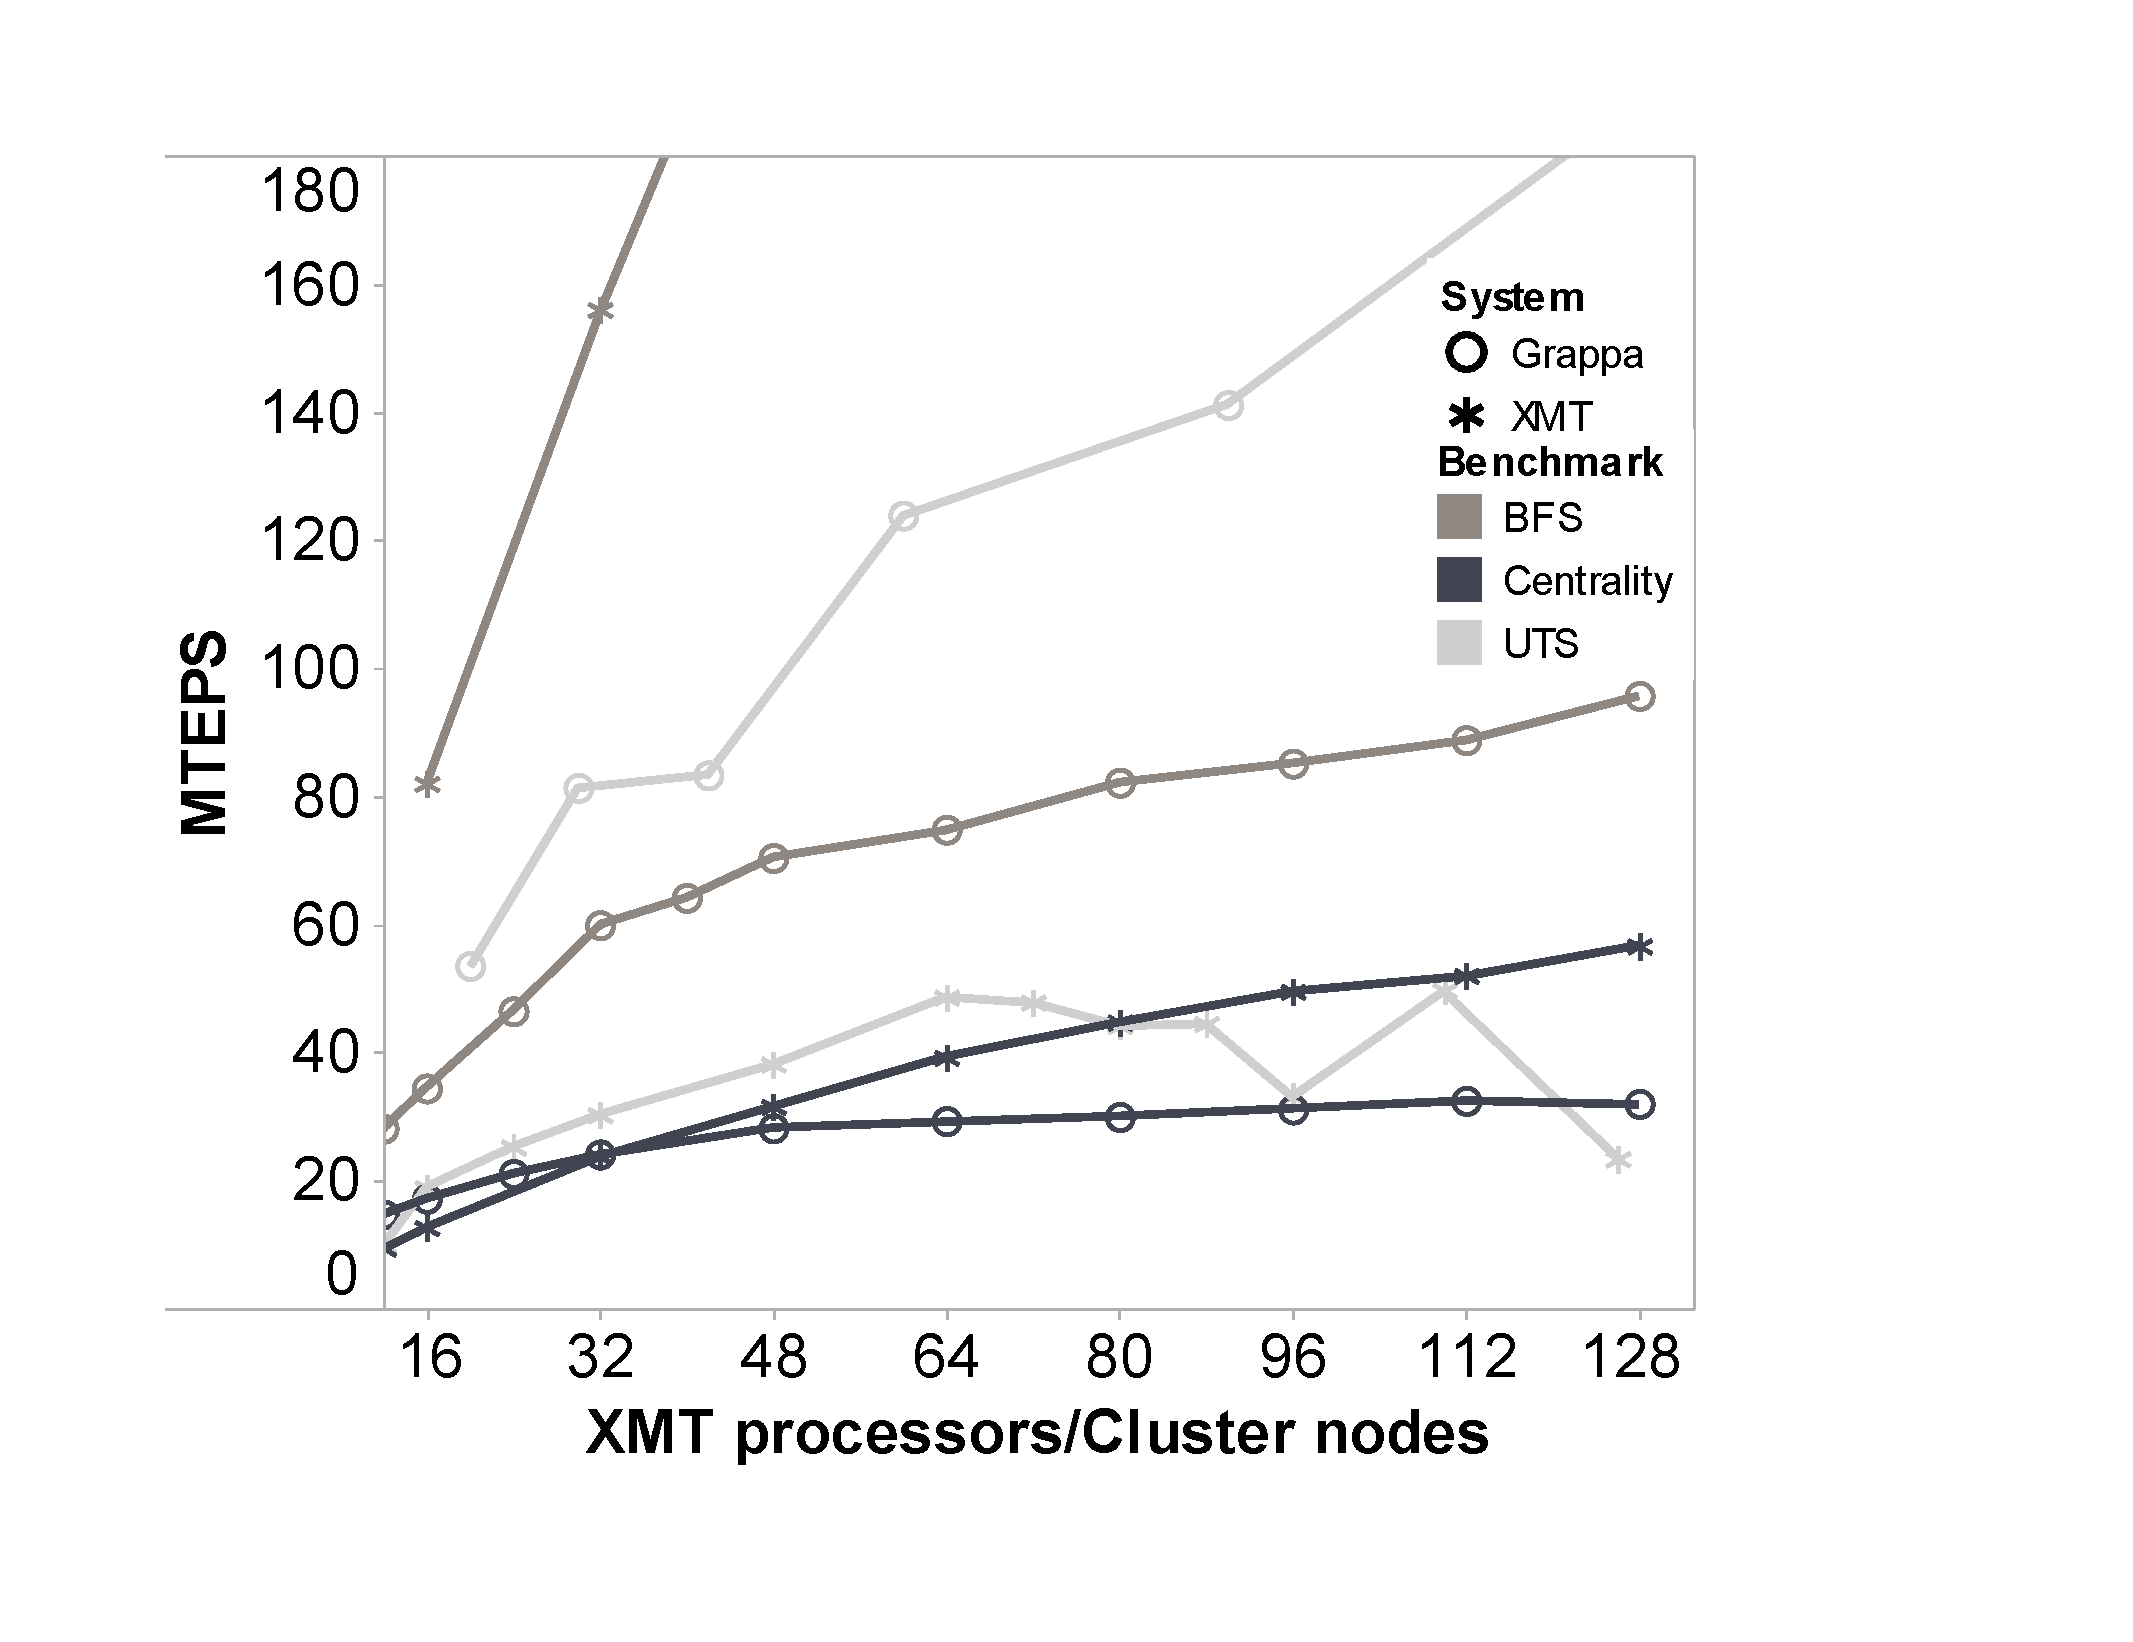
\includegraphics[width=0.5\textwidth]{figs/scaling_cropped.pdf}
    \end{center}
    \caption{Scaling number of nodes: \Grappa continues to perform significantly better than XMT for UTS but scales a constant factor slower than XMT for BFS (4x slower) and Centrality (2x slower). }
    \label{fig:uts_threshold}
\end{figure}


\subsection{Sensitivity}

\paragraph{Aggregator timeout}

\begin{figure}[htb]
\begin{center}
  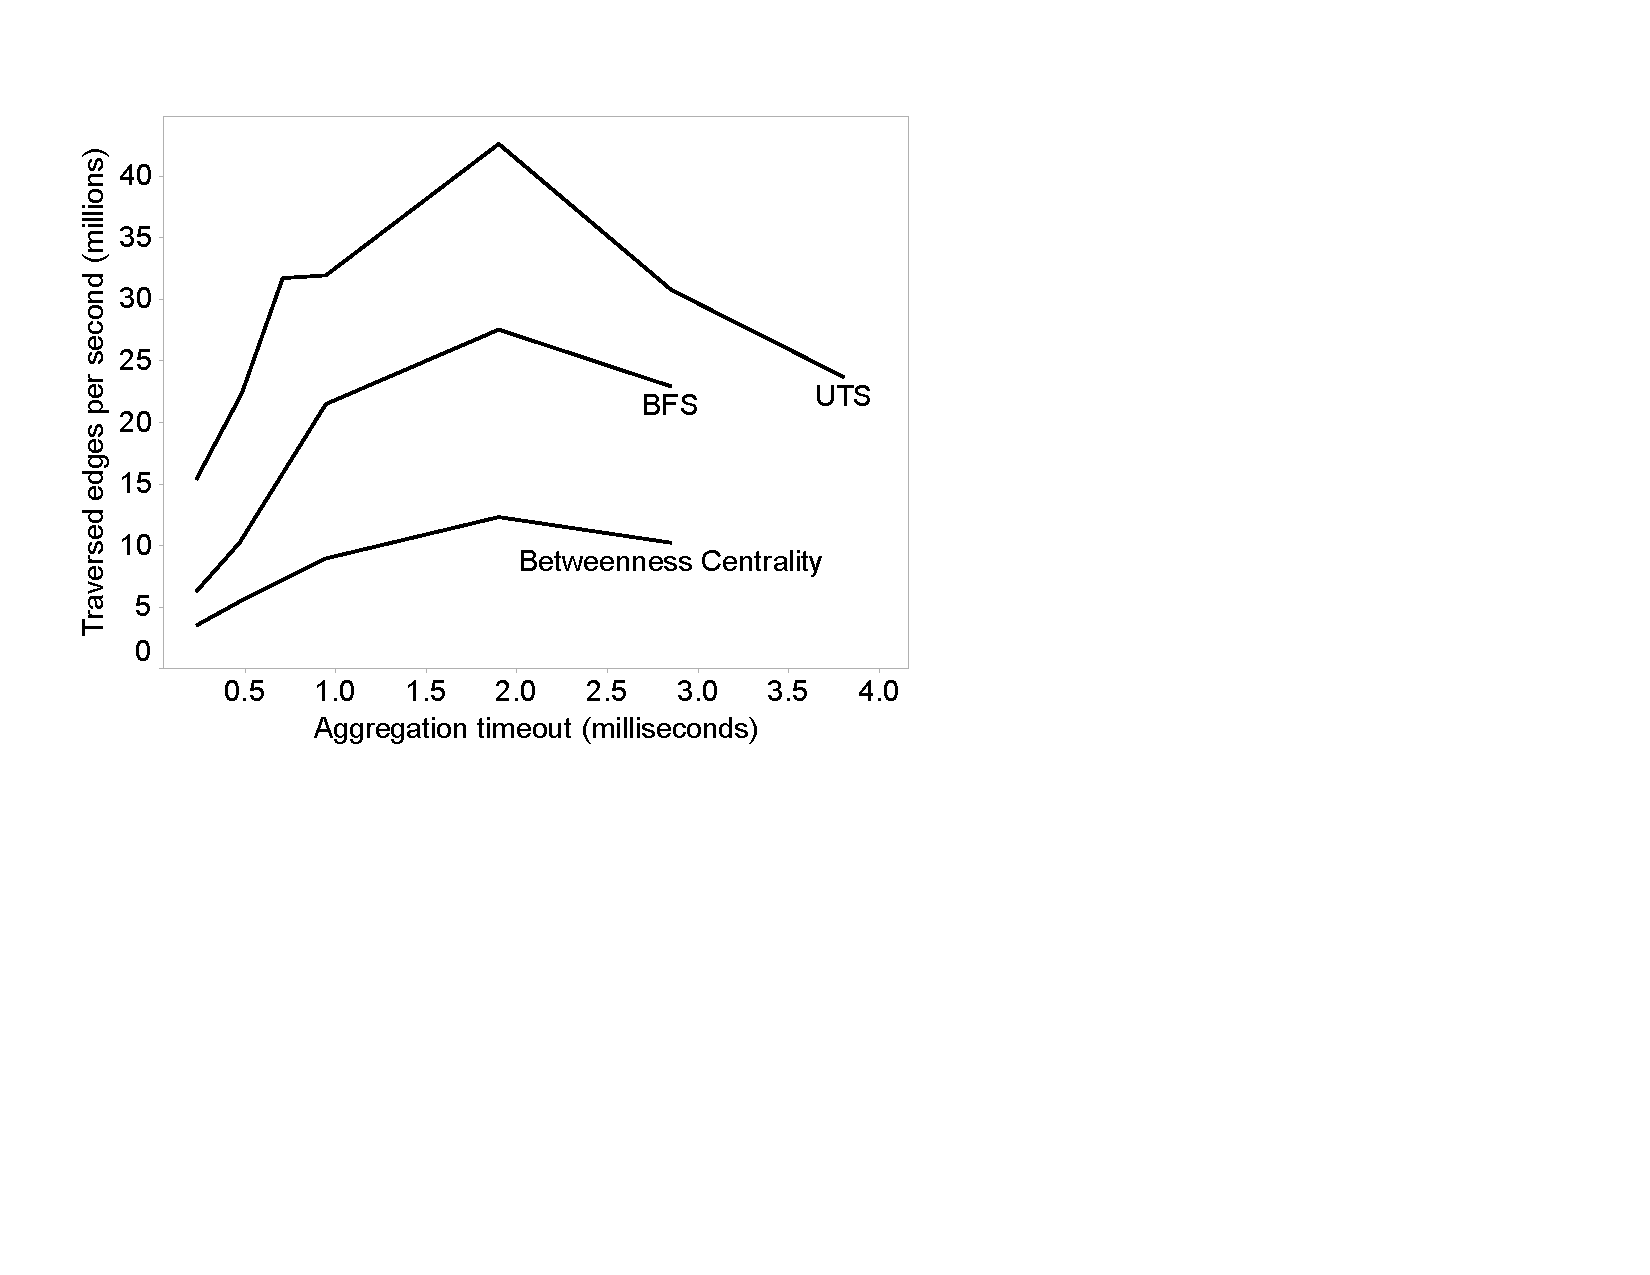
\includegraphics[width=0.95\columnwidth]{figs/flushticks_sweep}
\begin{minipage}{0.95\columnwidth}
  \caption{\label{fig:bfs-sweep-flushticks} Sensitivity to aggregation delay}
\end{minipage}
\vspace{-3ex}
\end{center}
\end{figure}


One of the key parameters of the aggregator is the message
timeout. All messages that are queued must eventually be sent in order
to ensure progress. In the best case, we are able to aggregate enough
messages to fill an aggregation buffer and cause it to be sent, but as
we scale up, the average rate of messages heading to a common
destination decreases, and this gets harder. To bound the problem, the
aggregator includes a timeout. Any packet waiting this long is sent
the next time the communications layer is serviced.

Figure~\ref{fig:bfs-sweep-flushticks} shows a sweep of this parameter
for UTS, BFS, and Betweenness Centrality on 16 nodes, using the
datasets described previously. The maximum number of workers is fixed
at 2048. All the benchmarks show a performance peak with a 2
millisecond timeout; at this point we are delaying long enough to
aggregate the largest packets we can; setting the parameter higher
causes tasks to wait longer for responses, but few new requests are
being generated.


\begin{figure}[htb]
\begin{center}
  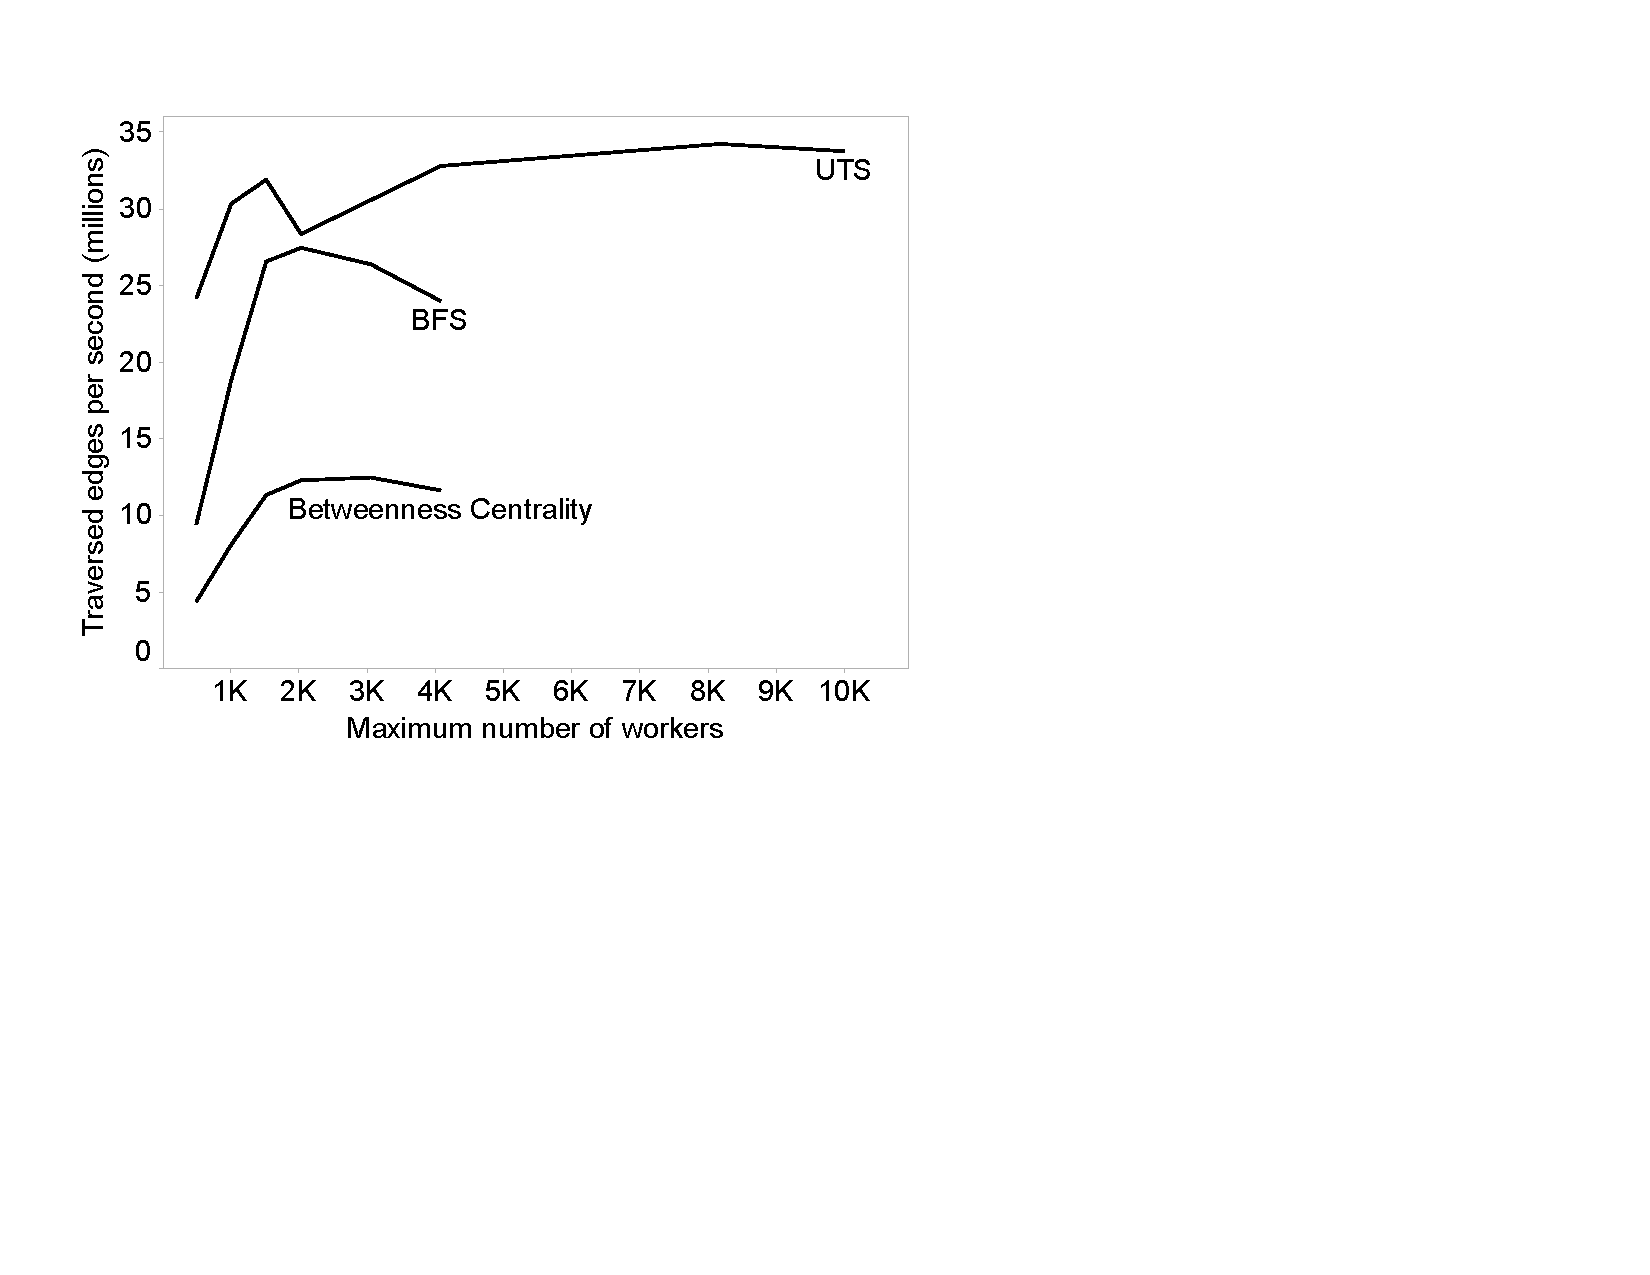
\includegraphics[width=0.95\columnwidth]{figs/worker_sweep}
\begin{minipage}{0.95\columnwidth} 
  \caption{\label{fig:bfs-sweep-workers} Sensitivity to maximum active tasks}
\end{minipage}
\vspace{-3ex}
\end{center}
\end{figure}

\subsubsection{Number of active tasks} \TODO{possibly eliminate}

When a task issues a request that requires a response, it blocks to
allow other tasks to utilize its core. These tasks may also block. To
support the many milliseconds of latency aggregation adds, we need to
support many thousands of blocked tasks. One of the key parameters of
the runtime is the number of blocked tasks allowed; we need enough to
cover the network and aggregation latency, but too many running tasks
can add extra latency as they all must be multiplexed onto the same core.

Figure~\ref{fig:bfs-sweep-workers} shows a sweep of the maximum number
of active tasks (workers) per core for each of our three benchmarks on
16 nodes. The aggregator timeout is set at 1 ms for UTS and 2 ms for
BFS and Betweenness Centrality. The performance peak shifts in this
case, with UTS peaking at 1536 workers, BFS peaking at 2048 workers,
and Betweenness Centrality peaking at 3072 workers. This is the point
where we have enough workers to cover the latency of aggreation. The
different values reflect the different amounts of work done by a task
in each benchmark; UTS does the least, while Betweenness Centrality does the most.

%\subsubsection{Work stealing parameters}
%
%\paragraph{Chunk size}
%
%It is important to steal multiple tasks at a time to both amortize the
%cost of stealing over the network and to spread out work quickly in a
%large system. Figure~\ref{fig:ut_chunksize} shows performance and
%stealing statistics for UTS on \checkme{30} nodes as we increase the stealing chunk size. Recall
%that a thief will take a number of tasks equal to the minimum of half
%the available work or the chunk size; steals fail only when the victim
%has fewer than 2 available tasks. As the scheduler is allowed to
%steal more work beyond 1 task, we see that performance increases up to 6x. This
%shows that the heuristic of stealing the oldest task from victims is
%insufficient alone when a tree-structured computation is imbalanced,
%as observed in \cite{UTS}. By observing sampled state in the execution
%trace, we find that a chunk size as low as 1 allows stealing to
%spread the load evenly across the cluster but cores spend much time
%underutilized as multiple workers wait for steal replies that
%utlimately return little new work.
%
%Performance plateaus before maximum steal amount is limited by the
%size of the victim's task queue. This indicates that artificially limiting steals
%to \checkme{128} tasks does not limit performance. Although a lower
%chunk size limits how quickly work spreads, for sufficient chunk size,
%the heuristic of stealing the oldest tasks from victims in tree-based computations allows for
%stolen work to expand quickly.


%% UTS: chunk size
%\begin{figure}[ht]
%    \begin{center}
%      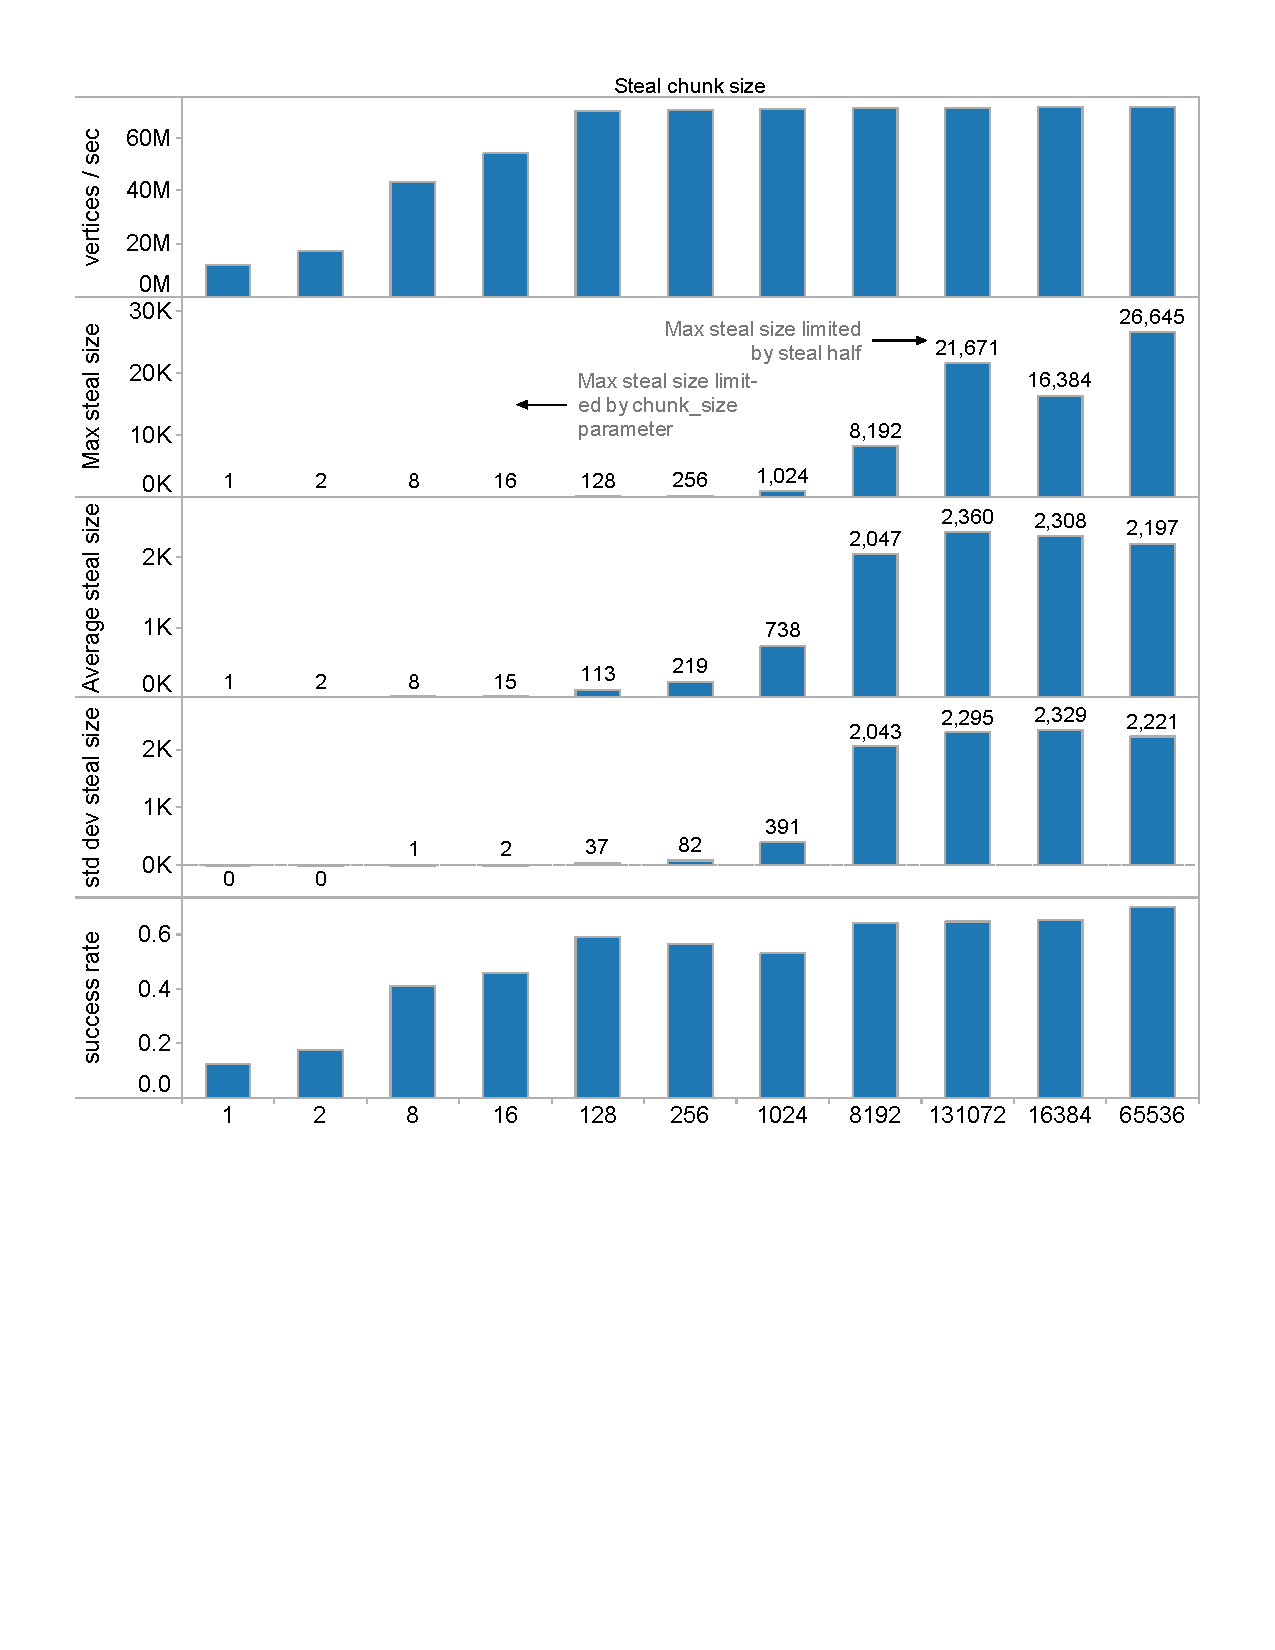
\includegraphics[width=0.5\textwidth]{figs/uts_chunksize.pdf}
%    \end{center}
%    \caption{Performance of UTS-Mem with varying maximum chunk size of
%    steals, run with 30 nodes, 6 cores per node, 4000 workers,
%    \checkme{6M flush ticks}}
%    \label{fig:uts_chunksize}
%\end{figure}


%\TODO{(difference with BFS)}



\subsubsection{Parallel loop threshold}

%\begin{figure}[htb]
%\begin{center}
%  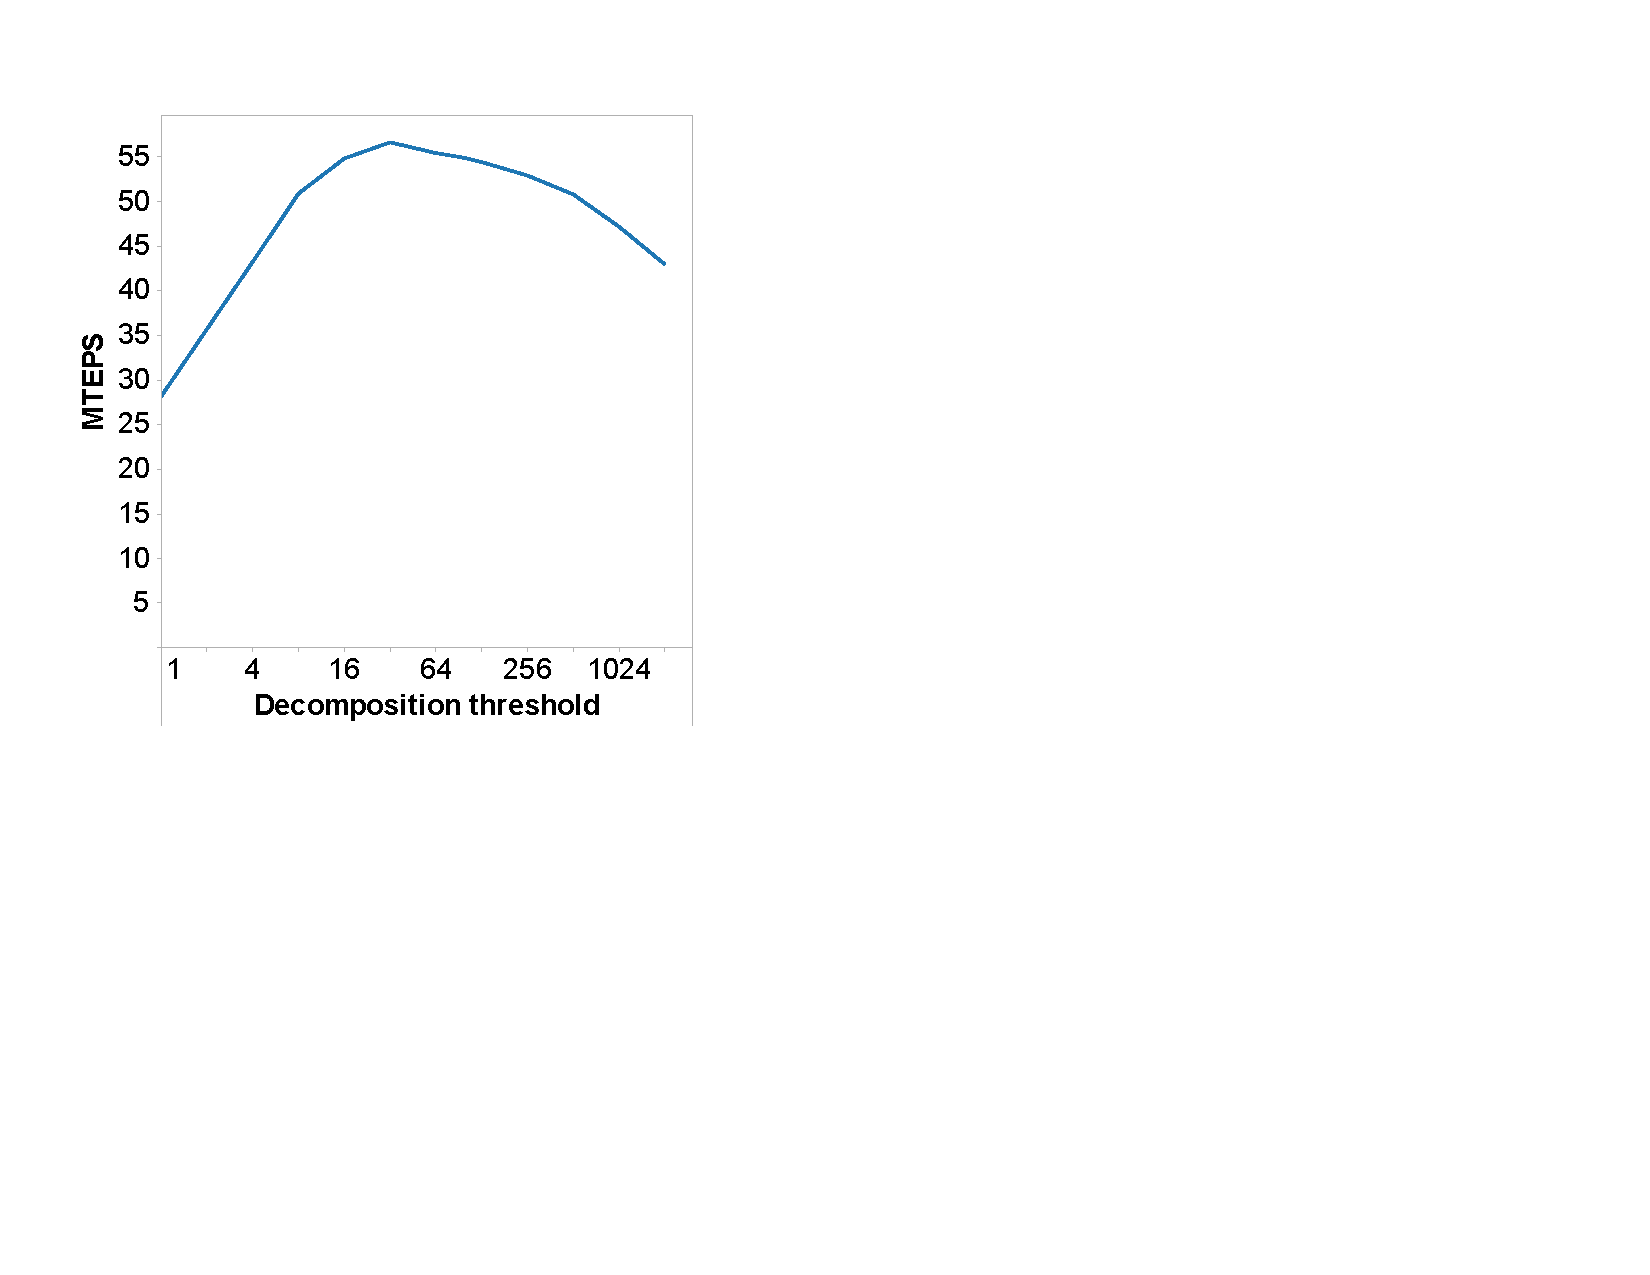
\includegraphics[width=0.95\columnwidth]{figs/bfs_sweep_threshold}
%\begin{minipage}{0.95\columnwidth}
%  \caption{\label{fig:bfs-sweep-threshold} Sensitivity to parallel loop threshold. Note the log scale.}
%\end{minipage}
%\vspace{-3ex}
%\end{center}
%\end{figure}

Parallel overhead---in the form of context switches, task spawns, and
synchronization---can reduce the performance benefit of parallelism.
\Grappa sees a benefit to limiting the amount of parallelism created by
a recursive loop decomposition. The parallel loop threshold (``parallel
granularity'') parameter tells the runtime when to stop creating new tasks and just execute iterations
sequentially. This allows us to amortize the overhead of task
creation. In addition, assigning sequential iterations to a single
task provides the potential to exploit locality when data for adjacent iterations is
also adjacent in memory. The ability to exploit this locality that
exists in the application is an important advantage. We found that in UTS and BFS, increasing the
threshold from 1 up to 8 or 16, respectively, increases performance by
more than 60\%.


% uts threshold
%\begin{figure}[ht]
%    \begin{center}
%      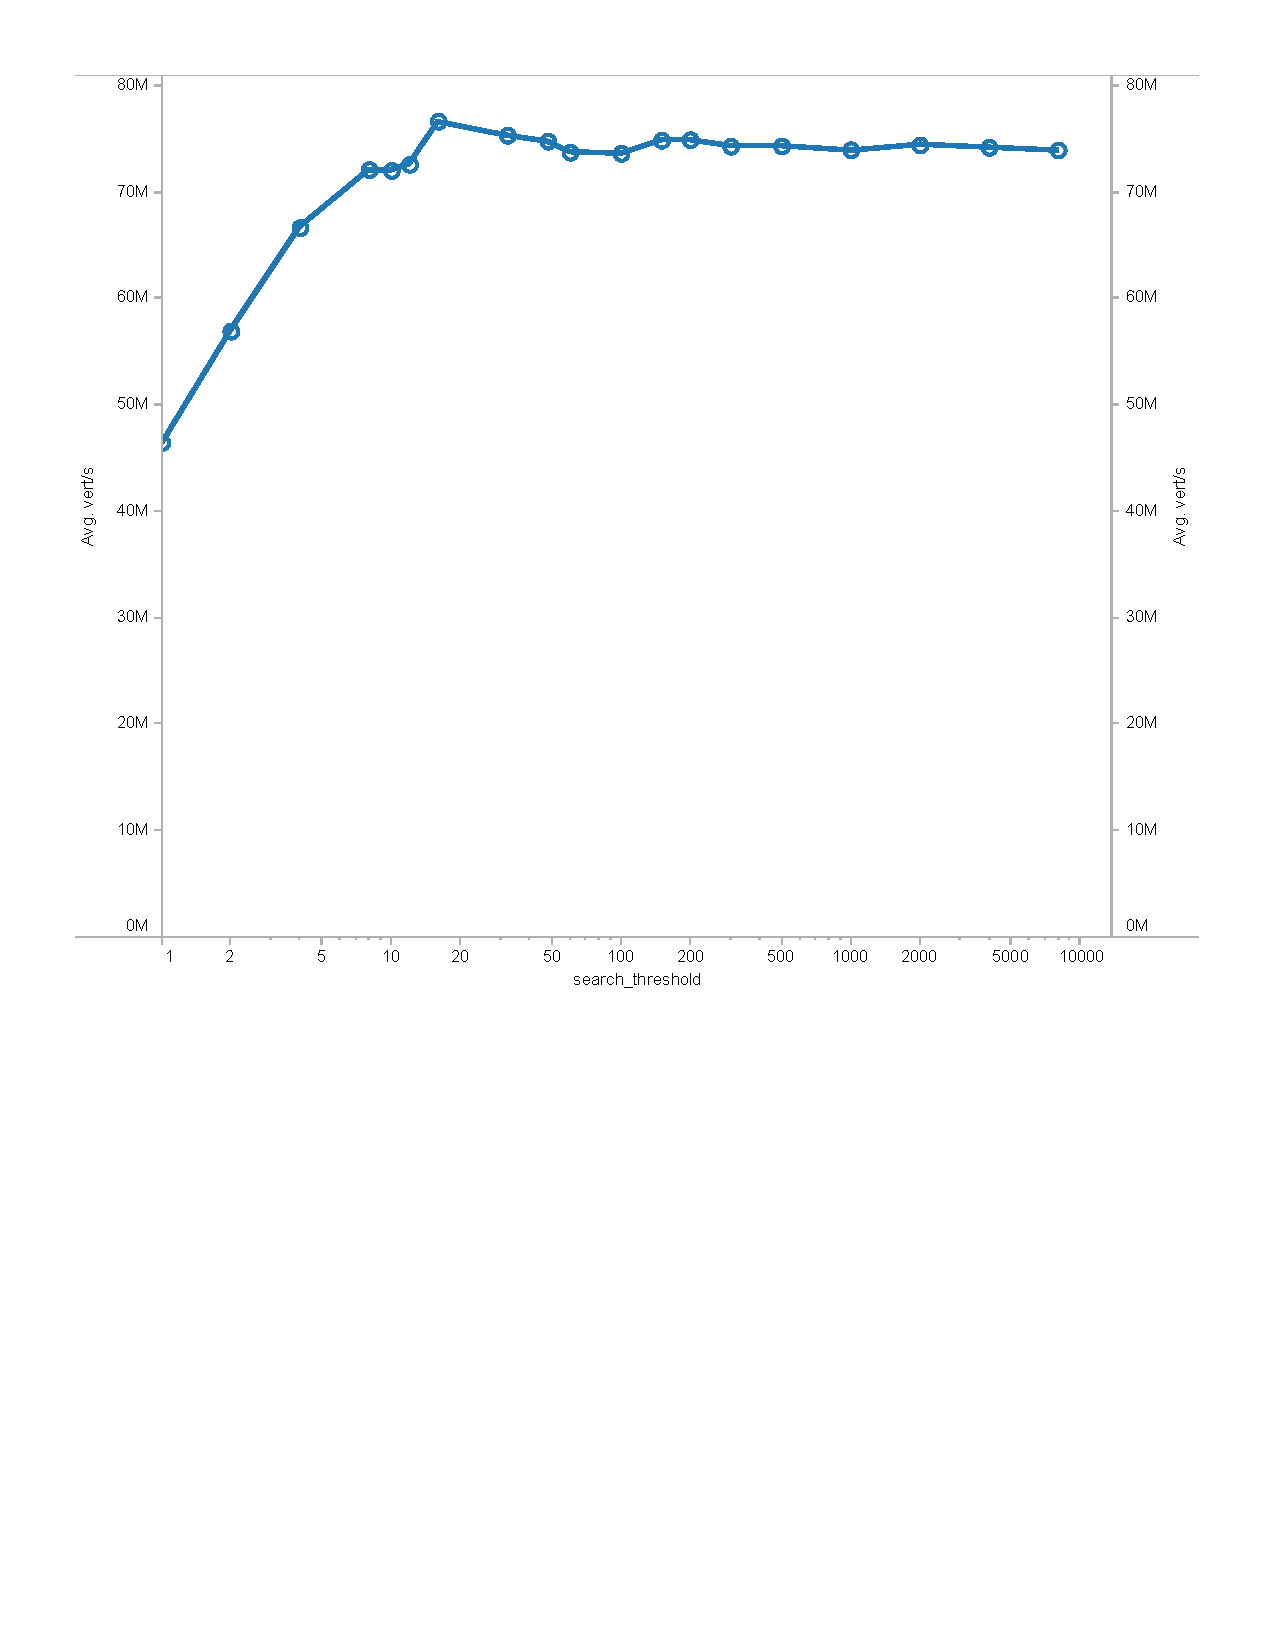
\includegraphics[width=0.5\textwidth]{figs/uts_threshold.pdf}
%    \end{center}
%    \caption{Performance of UTS-Mem with varying parallel loop
%        threshold, run with 30 nodes, 6 cores per node, 4000 workers,
%    \checkme{6M flush ticks}}
%    \label{fig:uts_threshold}
%\end{figure}

\subsection{Summary}\TODO{this is a placeholder: do we need this section?}

\paragraph{Context-switch overhead.} Should we also compare with other packages? (Maybe Capriccio, QThreads?, or even real OS threads?)

\paragraph{Latency.} Measure remote data access latency with and without aggregation turned on.

\paragraph{Aggregated message sizes.} Characterization of the resulting message sizes with aggregation. Right now we only have message size vs. bandwidth.

\paragraph{Utilization.} CPU utilization, Memory, Network. It would be great to answer the question of where is our bottleneck right now. Amount of concurrency with and without aggregation. 

\paragraph{Memory accesses.} Rate of accesses to remote data. Rate of delegate ops. Show limit with GUPs.



%Retries are performed by the memory controller when remote synchronization operations fail to find the full-bit associated with each memory location in the unavailable state.  Retries are issued at low priority relative to new memory operations issued by the processor by other contexts, so they consume what would otherwise be unused injection bandwidth.  On a full-bandwidth system such as the MTA-2, retries have no impact on the progress of tasks other than their own.  On a Cray XMT, network bandwidth is limited, so retries create congestion.  In comparison, \Grappa performs synchronization without retries, delaying responses at the receiving end until ready to notify the sender to proceed.  This saves bandwidth and permits scaling of tasks performing synchronization even on low injection rate networks.


%\begin{figure*}[ht]
%    \begin{minipage}{0.3\linewidth}
%        \centering
%        \includegraphics[width=\textwidth]{figs/chunksize-uts.pdf}
%        \caption{chunksize caption}
%        \label{fig:chunksize-uts}
%    \end{minipage}
%    \begin{minipage}{0.3\linewidth}
%        \centering
%        \includegraphics[width=\textwidth]{figs/workers-uts.pdf}
%        \caption{workers caption}
%        \label{fig:workers-uts}
%    \end{minipage}
%    \begin{minipage}{0.3\linewidth}
%        \centering
%        \includegraphics[width=\textwidth]{figs/thresh-uts.pdf}
%        \caption{threshold caption}
%        \label{fig:thresh-uts}
%    \end{minipage}
%\end{figure*}

}

\todo{End eval insert}

current: just context switch on single node


linked lists:

there is some room for memory concurrency

thread contexts don't take up too much space in cache

sparse matmul:

speedup?






\section{Related work}


hardware:

XMT/MTA

cyclops

niagra

software:

qthreads

cilk? tbb?

why not wait for more cores?

hyperthreading?



\section{Conclusion}

Large irregular problems found in areas such as social networking and
bioinformatics tend to have poor performance on commodity clusters due
to frequent low-locality memory accesses. We present a programming
model and runtime system that uses lightweight context switching to
tolerate long-latency accesses and increase performance on these
applications. Our preliminary evaluation shows that the overhead of
context switching is not prohibitive for thread counts needed for a
large-scale implementation, but memory concurrency is limited by
hardware structures in commodity processors. We describe how we plan
to address the challenges of large-scale memory concurrency and
lightweight synchronization.


\bibliographystyle{acm}
\bibliography{softxmt-hotpar2011}

\end{document}
